\hypersetup{pageanchor=false}
\part{Introduction}
\hypersetup{pageanchor=true}

\chapter{Overview}
\label{chapter:overview}
\glsresetall

\section{High-Dimensional Data Stream Mining}

\subsection{Knowledge Discovery from Data}
% See for example https://machinelearningmastery.com/what-is-data-mining-and-kdd/

Data Mining, also referred to as \gls{KDD}, is known in the community as the process of extracting useful patterns from massive data repositories, such as large databases, data warehouses, or data streams \cite{DBLP:books/mk/HanKP2011}. The \gls{KDD} process usually serves as a reference for the required steps of any data analysis task and draws the plan of most textbooks in the field \cite{DBLP:books/sp/DM2005, DBLP:books/mk/HanKP2011,kantardzic2011data,DBLP:books/sp/Aggarwal15}. In Figure~\ref{fig:KDD}, we represent this process, which consists of seven steps, with multiple feedback loops: 
\begin{enumerate}[noitemsep]
	\item \textbf{Data Cleaning}: Removing noise and inconsistency in the data.
	\item \textbf{Data Integration}: Combining multiple data sources into a Data Warehouse.
	\item \textbf{Data Selection}: Selecting the observations/attributes relevant to the task at hand.
	\item \textbf{Data Transformation}: Transforming the data into a format adequate for further analysis (e.g., deriving new features and aggregates from the existing attributes).
	\item \textbf{Data Mining}: Using specific algorithms to extract patterns from data. Examples of potentially interesting patterns are groups of frequent items, clusters or outliers. 
	\item \textbf{Pattern Evaluation}: Filtering the patterns found in the previous step by identifying the most valuable ones for a given task, e.g., based on a set of quality criteria.
	\item \textbf{Knowledge Representation}: Representing the patterns via representation and visualisation methods to make them interpretable for the users. 
\end{enumerate} 

The \gls{KDD} process typically is treated as a cyclic pipeline, in which the knowledge gained over each iteration helps to improve the execution of each step.

\begin{figure}[ht]
	\centering
	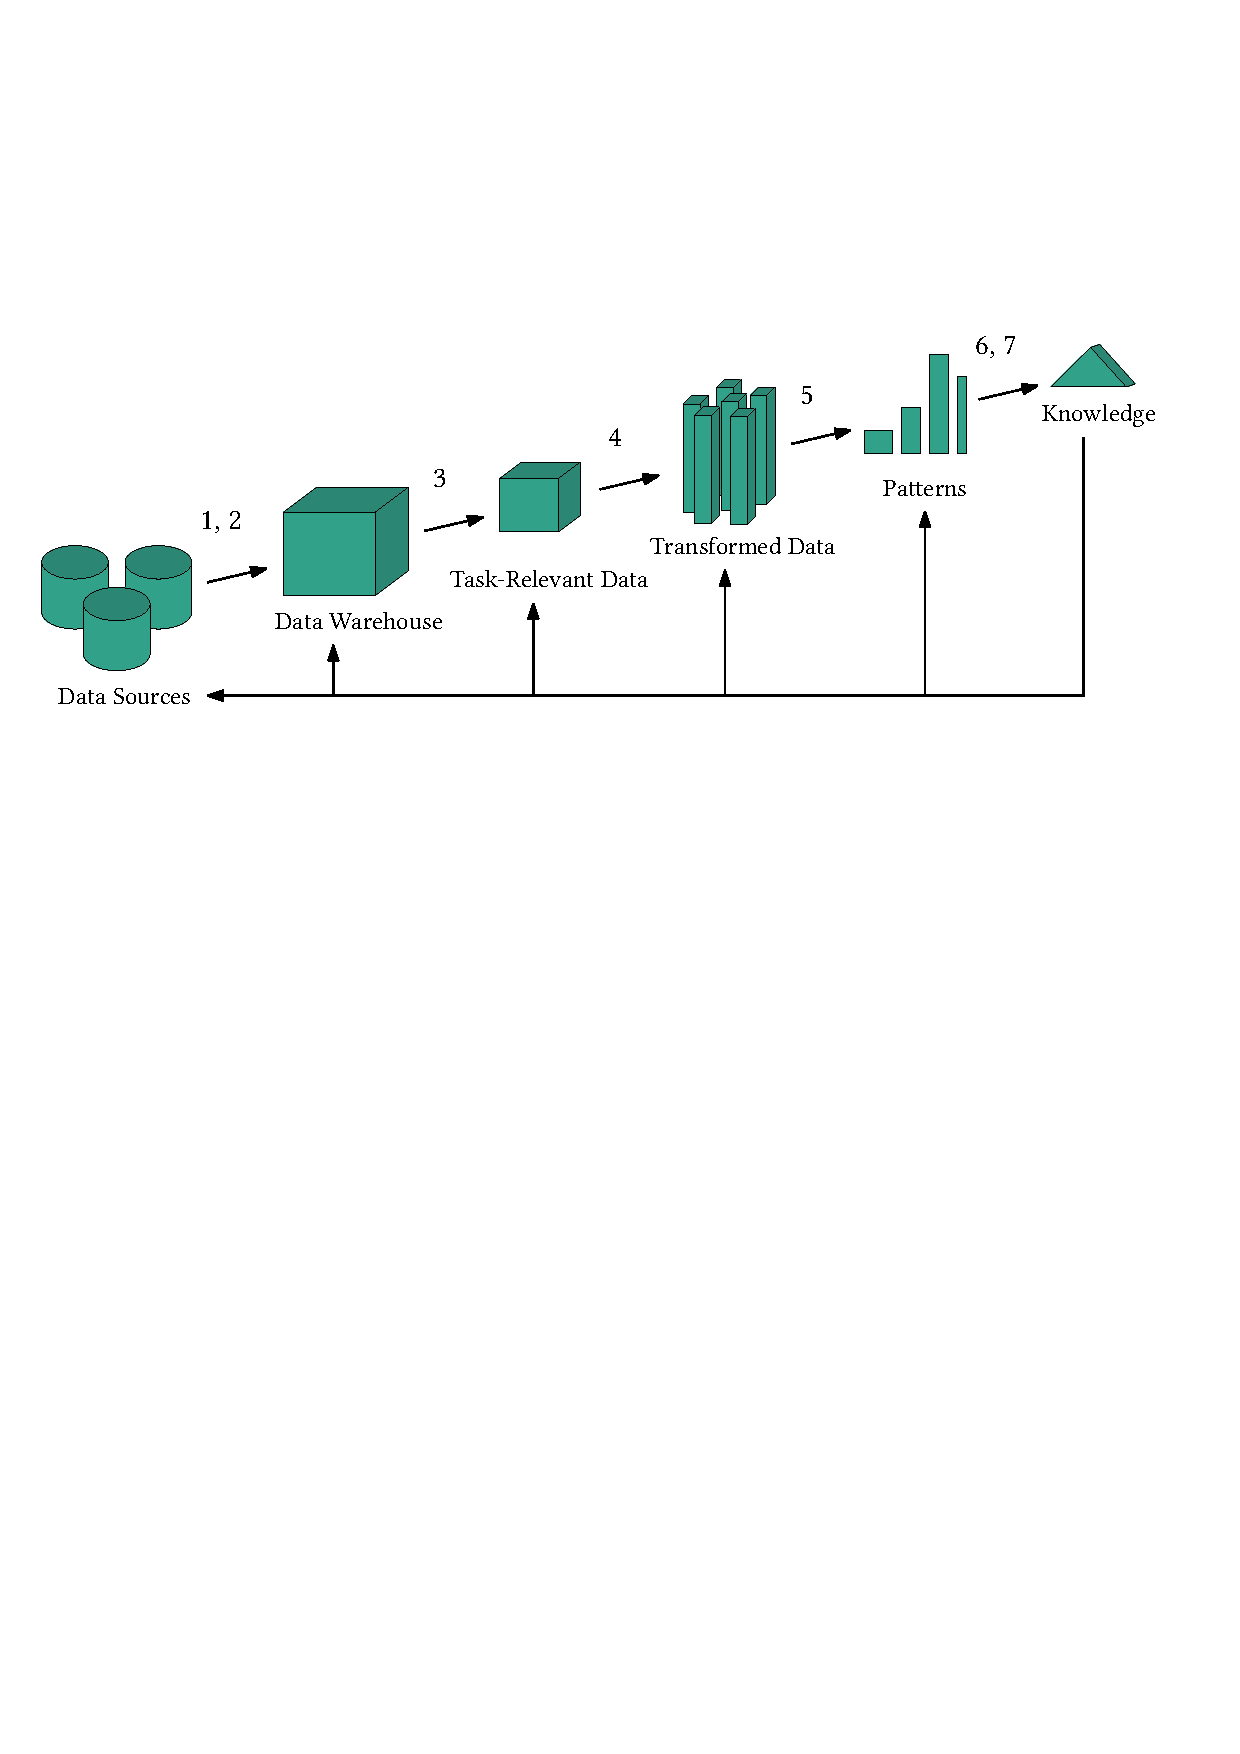
\includegraphics[width=0.95\textwidth]{part1-figures/kdd-compressed.pdf}
	\caption{\acrfull{KDD}, according to \cite{DBLP:books/mk/HanKP2011}.}
	\label{fig:KDD}
\end{figure} 

As we can see, Data Mining also refers to the core step of this process (Step 5). The literature uses the term Data Mining interchangeably with \gls{KDD}, perhaps for conciseness \cite{DBLP:books/mk/HanKP2011}. In turn, the community usually describes Data Mining as a discipline at the frontier of multiple fields: Database Management, Artificial Intelligence, Machine Learning, Pattern Recognition, Data Visualisation. In this dissertation, we refer to Data Mining or Knowledge Discovery as the whole process and leave the debate on the semantic differences w.r.t.\ Machine Learning, Data Science, etc., to the literature \cite{DBLP:books/aw/TanSK2005, Friedman97datamining}.

Researchers have examined every step of the process, and a wide range of methods is now available to extract patterns from data. 
%Note: At this point, we could have examples of for what Data Mining is useful for (but we have this in abstract now so I guess it's good enough)
However, Data Mining remains challenging under certain circumstances. In particular, when (1) the data is high-dimensional, i.e., it has many attributes, and when (2) the data comes as a stream. These two problems have raised the interest of the research community for years \cite{DBLP:journals/sadm/ZimekSK12,DBLP:books/sp/Aggarwal2013,DBLP:journals/ijon/Ramirez-Gallego17,DBLP:journals/pai/Gama12}. While the literature separately addressed them to some extent, the intersection of both has received less attention. For example, recent clustering  \cite{DBLP:journals/csur/SilvaFBHCG13,DBLP:books/daglib/0030859,DBLP:journals/jcst/AminiTS14,DBLP:journals/ijon/WuLH12} or prediction  \cite{DBLP:conf/ijcai/TanTL11,DBLP:conf/aaai/WangRNBMX17,DBLP:journals/sadm/ZimekSK12,DBLP:conf/dasfaa/AssentKBS12,DBLP:conf/icdm/SatheA16,DBLP:conf/sdm/ChenSAT17} algorithms tend to tackle at most one of those aspects: either high-dimensionality restricted to static data, or the streaming scenario, limited to few variables. 
The difficulty is that both the high-dimensionality and the streaming setting come with distinct sets of challenges. 

Data Mining at the intersection of both problems remains mostly unaddressed \cite{DBLP:journals/sigkdd/SalehiR18}, i.e., there is a gap in the current research landscape (Figure~\ref{unexplored}). While one option is to extend or invent specific methods for high-dimensional data streams, as in \cite{DBLP:conf/icde/ZhangGW08, DBLP:conf/sdm/NtoutsiZPKK12}% see also \cite{ DBLP:conf/vldb/AggarwalHWY04,  DBLP:conf/icde/ZhangGW08, DBLP:conf/icde/CaoYWYWR14}, % DBLP:conf/ssdbm/HassaniKSS14, 10.1145/3219819.3220107
, a perhaps more general -- but not less effective -- contribution is to develop fundamental tools for Knowledge Discovery in this particularly challenging setting. 

This observation forms the starting point of our dissertation. We bridge this gap by proposing algorithms to address both sets of challenges. We start with a fundamental task: dependency estimation. We show that, combined with efficient monitoring techniques, our algorithms support further Knowledge Discovery in high-dimensional data streams.

\begin{figure}
	\centering
	\begin{tikzpicture}[thick]
	
	\begin{scope}
	\clip (2.5,2) circle (2.5cm);
	\fill[pattern=crosshatch, pattern color=uiucred] (6.5,2) circle (2.5cm);
	\end{scope}
	\draw (2.5,2.25) node { High};
	\draw (2.5,1.75) node { Dimensionality};
	\draw (2.5,2) circle (2.5cm);
	
	\draw (6.5,2) circle (2.5cm);
	\draw (6.5,2.25) node { Data};
	\draw (6.5,1.75) node { Streams};
	
	\end{tikzpicture}
	\caption{A gap in the Data Mining research landscape.}
	\label{unexplored}
\end{figure}

In the remaining of this chapter, we detail the challenges associated with high-dimensionality and data streams. Then, we show that the task of dependency estimation is critical to most Data Mining applications and present our running use case: the \acrshort{Bioliq} power plant. Finally, we detail our contributions and the outline of this dissertation.  

\subsection{Challenges of High-Dimensionality}
\label{challenges:highdimensionality}

When the data is high-dimensional, several effects, summarised as the \textit{curse of dimensionality} \cite{bellman1957}, bog down the performance of traditional statistical approaches \cite{DBLP:conf/icdt/BeyerGRS99}. 

A linear increase in the number of dimensions in the euclidean space leads to an exponential increase in volume. The space becomes extremely sparse, and the distances between each pair of points converge to the same value. This effect is known as \textit{distance concentration}. \cite{DBLP:conf/icdt/BeyerGRS99} showed that, under broad conditions, the probability that the minimum $\mathcal{D}_{\text{min}}^n$ and the maximum distance $\mathcal{D}_{\text{max}}^n$ differ by a factor smaller than $1 + \epsilon$ converges to $1$ as the number of dimensions $n$ increases, i.e., 
\begin{align}
\lim_{n \rightarrow \infty} \Pr\left[\mathcal{D}_{\text{max}}^n \leq (1 + \epsilon) \cdot \mathcal{D}_{\text{min}}^n\right] = 1, \quad \forall \epsilon > 0. 
\end{align} 

Figure~\ref{fig:cod} illustrates this via simulation. We report the maximum, average and minimum euclidean pairwise normalised distances within $100$ \textit{i.i.d.} observations in $\mathcal{U}[0,1]$. We average the results over $1000$ independent trials; The coloured areas show the standard deviation. As we can see, the distances converge as $n$ increases. Thus, in high-dimensional spaces, observations tend to be equally far from each other. The performance of most Data Mining algorithms, which rely on local neighbourhoods, drastically decreases.  

\begin{figure}
	\centering
	\subfigure[The \textit{distance concentration} effect]{
		\label{fig:cod}
		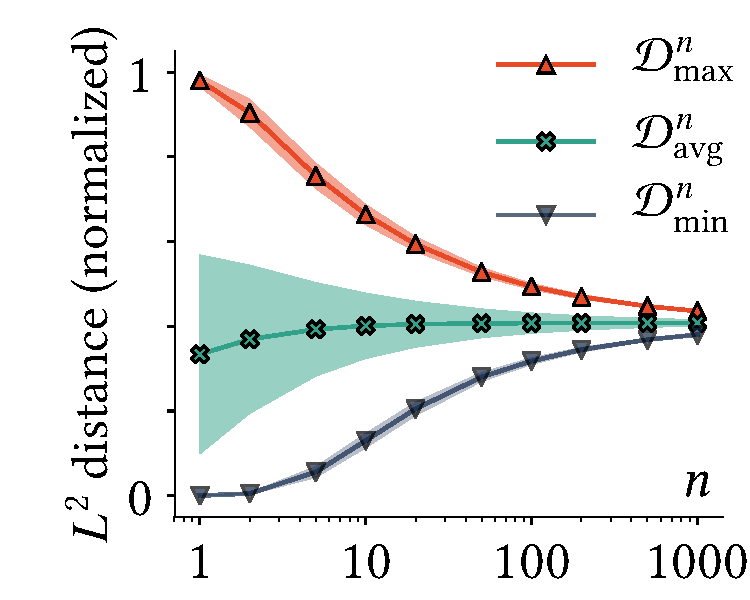
\includegraphics[width=0.36\linewidth]{part1-figures/cod_illustration-compressed.pdf}
	}
	\hfill
	\subfigure[Number of pairs]{
		\label{fig:cod_pairs}
		\begin{tikzpicture}[thick]
		\begin{axis}[width=0.34\textwidth, height=0.35\textwidth, axis lines=middle,xlabel=$n$,enlargelimits,
		scaled y ticks={base 10:-3}] 
		\addplot[domain=2:100, color=uiucblue] {x*(x-1)/2} node[left]{$f(n) = \frac{n \cdot (n-1)}{2}$};
		
		\end{axis}
		\end{tikzpicture}}
	\hfill
	\subfigure[Number of subspaces]{
		\label{fig:cod_subspaces}
		\begin{tikzpicture}
		\begin{axis}[width=0.34\textwidth, height=0.35\textwidth, axis
		lines=middle,xlabel=$n$,enlargelimits] 
		\addplot[domain=2:20, color=uiucred] {2^x - 1} node[left]{$g(n) = 2^n - 1$};
		\end{axis}
		\end{tikzpicture}}
	\caption{Illustration of the effects of the \textit{curse of dimensionality}.}
	\label{fig:searchspace}
\end{figure}
%Note: "Conventional method such as Kernel Density Estimation (KDE) performs poorly for high-dimensionaldata (d >3)." -> Nonparametric Density Estimation for High-Dimensional Data - Algorithms and Applications (Zhipeng Wang∗and David W. Scott)
% Source saying that density estimation in high-dimensional space does not work -> Scott (Multivariate Dependency Estimation, page 202)

A common workaround consists in restricting the analysis to small sets of attributes (subspaces) of interest, e.g., via \textit{dimensionality reduction} methods. 
However, \textit{dimensionality reduction} also is challenging: the number of pairs for a number $d$ of attributes is $\frac{n \cdot (n-1)}{2}$ for symmetric measures (Figure~\ref{fig:cod_pairs}), while the number of subspaces is $2^n - 1$ (Figure~\ref{fig:cod_subspaces}). As a result, they grow quadratically/exponentially with $n$, so that, even for a moderate amount of attributes, one cannot afford to investigate each attribute pair or subspace. 

For example, with $20$ attributes, the number of subspaces is already more than one million (Figure~\ref{fig:cod_subspaces}).
\cite{DBLP:books/sp/Aggarwal2013} famously compared the task of finding a pattern (e.g., an outlier) in high-dimensional spaces to that of searching for a needle in a haystack, while the haystack is one from an exponential number of haystacks. Subspace search methods, such as \cite{DBLP:conf/sdm/BohmKMNV13, DBLP:conf/bigdataconf/NguyenMB13, DBLP:conf/icde/KellerMB12, DBLP:journals/ijdsa/TrittenbachB19}, efficiently solve this problem to some extent. 

%The problem is that patterns, such as outliers, may only be visible within a few of those subspaces \cite{DBLP:conf/icde/KellerMB12}. 

We refer to \cite{DBLP:books/lib/HastieTF09} for further illustrations of the effect of the \textit{curse of dimensionality} and to \cite{DBLP:journals/sadm/ZimekSK12} for a discussion centred on outlier detection. 

\subsection{Challenges of Data Streams}
\label{challenges:datastreams}

In the real world, data often is a stream, i.e., data is collected online and may evolve in unforeseeable ways. In this setting, static approaches are ineffective \cite{DBLP:journals/pai/Gama12} because of changes in the data generation, characterised by a phenomenon known as \textit{concept drift}.

Thus, patterns are meaningful only in the right time context. For example, in Figure~\ref{fig:drift}, an observed outlier at time $T=1$ might not be relevant any more at time $T=2$ and vice-versa. Next, the scale of this time context also is unknown. In broader time contexts, e.g., $T=\{1,2,3\}$, the outliers may not be visible as such.

\begin{figure}
	\centering
	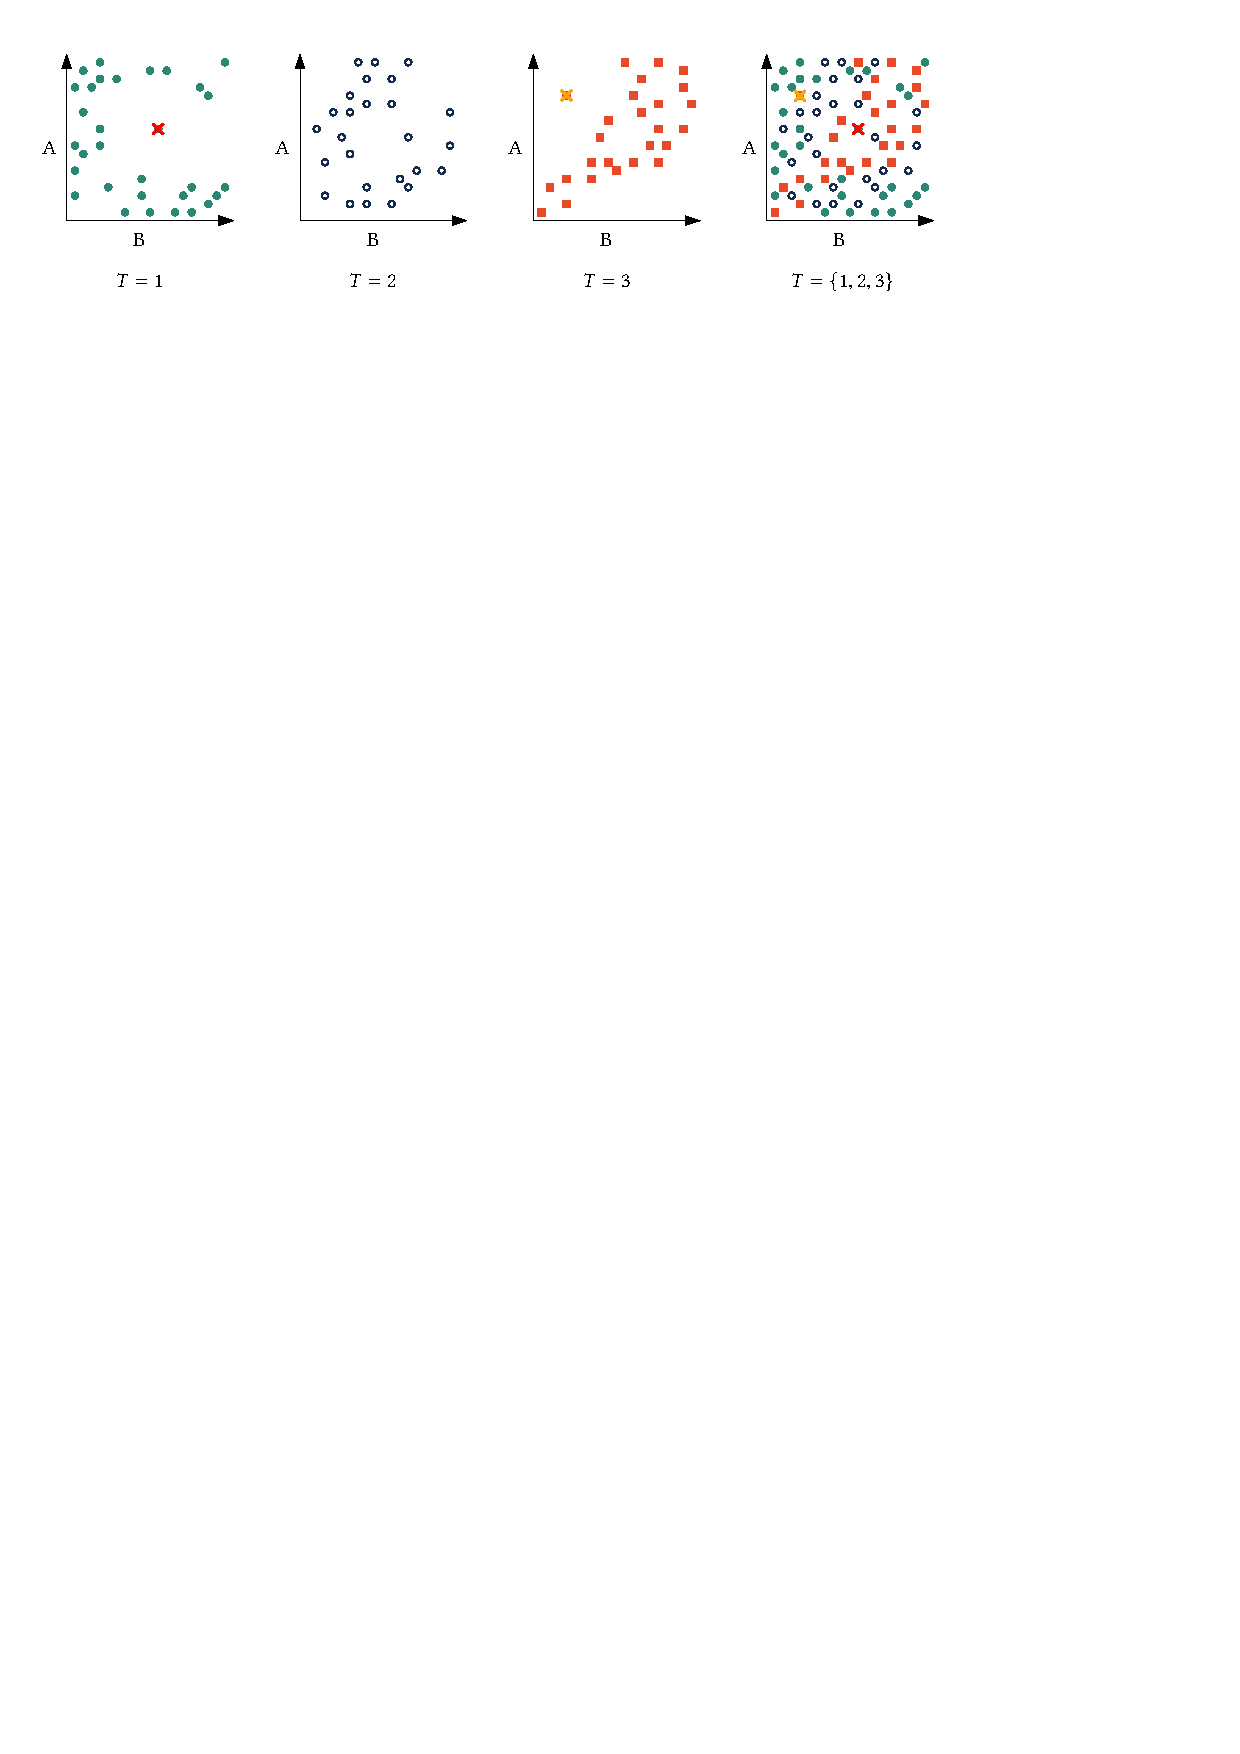
\includegraphics[width=1.0\textwidth]{part1-figures/time_example-compressed.pdf}
	\caption{Concept drift -- Patterns are only visible in their local context.}\label{fig:drift}
\end{figure} 

Data streams are subject to various types of \textit{concept drifts} \cite{DBLP:conf/ictai/BarddalGE15}, which can vary in speed and intensity and may also have seasonal components. 
The streaming nature of the data constrains system design in several ways, laid out by \cite{doi:10.1198/1061860032544} as follows:  
\begin{itemize}[noitemsep]
	\item \hypertarget{C1}{\textbf{Efficiency (C1):}}  The system must spend a short constant time and a constant amount of memory to process each incoming record.
	\item \hypertarget{C2}{\label{C2} \textbf{Single Scan (C2):}} The system may perform at most one scan over the data since access to past observations is often unavailable or impractical. 
	\item \hypertarget{C3}{\textbf{Adaptation (C3):}} Whenever the data distribution changes over time, the system must adapt, e.g., by forgetting outdated information.
	\item \hypertarget{C4}{\label{C4} \textbf{Anytime (C4):}} The system must be available at any point in time, with an output ideally equivalent (or nearly identical) to the one of a non-streaming system, operating without the streaming constraints. 
\end{itemize}   
The streaming scenario is particularly challenging because one needs to monitor the evolution of data. Data Mining algorithms must integrate an adequate forgetting mechanism to discard obsolete information and monitor the stream.

%Additionally, the high-dimensionality challenges the efficiency and effectiveness of streaming algorithms. In the end, the computational effort of existing methods generally is too high to allow for their deployment in real-time.

Furthermore, streams often consist of observations with various types, e.g., numerical, ordinal, or categorical. Such data sources are known as \textit{Heterogeneous Data Streams} \cite{DBLP:conf/icdm/YangZ06}. \cite{DBLP:journals/cim/DitzlerRAP15} identified mining from heterogeneous data as one of the most challenging problems of Data Mining. Thus, \textit{heterogeneity} adds up to the list of constraints above:
\begin{itemize}
	\item \hypertarget{C5}{\label{C5} \textbf{Heterogeneity (C5)}}: The system must handle not only numerical types but ideally all data types such as strings, categories, ordinal values. 
\end{itemize} 
The main challenge is to provide Data Mining techniques that can cope both with the streaming constraints and high-dimensionality -- our goal in this dissertation.  

\subsection{The Central Role of Estimating Dependency}
\label{sec:centralrole}

Dependency estimation is a fundamental technique in Data Mining \cite{DBLP:journals/tkde/ChenHY96} and consists of quantifying the strength of the statistical relationship between attributes, based on the available observations. It helps to find the relevant variables for the task at hand, which leads to a better understanding of data and improves both the runtime and the outcomes of downstream mining tasks, e.g., classification, outlier detection, or clustering.

To this end, dependency estimators such as the \textit{Pearson correlation coefficient}, or \textit{mutual information} \cite{DBLP:journals/bstj/Shannon48} as a non-linear counterpart, are perhaps the most well-known examples. Dependency estimation techniques are a building block of many Data Mining approaches, and play a role at every step of the process (see Figure~\ref{fig:KDD}), for example:
\begin{itemize}[noitemsep]
	\item \gls{EDM} \cite{DBLP:books/wi/DasuJ03, DBLP:journals/sigkdd/AssentKMS07, DBLP:conf/ieeevast/TatuMFBSSK12} is fundamental for \textbf{Data Cleaning} and \textbf{Data Integration}. \gls{EDM} reveals structures in the data, e.g., artefacts and inconsistencies that one should clean, or relevant attributes to integrate before subsequent analysis. Dependency estimators \cite{DBLP:journals/sigkdd/ParsonsHL04, DBLP:conf/vldb/ZhuS02, DBLP:conf/sigmod/MayfieldNP10} are a characteristic tool of \gls{EDM} to discover such structures.  
	\item Filtering out the attributes irrelevant for the task at hand is key to deal with high-dimensionality. \textit{Feature Selection} \cite{DBLP:journals/jmlr/GuyonE03} methods are critical for \textbf{Data Selection} and heavily rely on dependency estimators \cite{DBLP:journals/pami/PengLD05, DBLP:journals/tkde/HallH03, DBLP:journals/eswa/BennasarHS15, DBLP:journals/pr/LiuSLZ09}. 
	\item \textbf{Data Transformation}, also known as \textit{Feature Engineering}, consists in transforming the data into an adequate format, and possibly enhancing the original data with additional features. Dependency estimates can be used as feature to improve the results of downstream analysis \cite{DBLP:conf/vldb/ZhuS02, DBLP:journals/jmlr/Torkkola03, DBLP:conf/icml/YuanH09, DBLP:conf/eenergy/VollmerETBKB19}. 
	\item Numerous \textbf{Data Mining} algorithms, e.g., clustering \cite{DBLP:conf/sdm/BohmKMNV13, DBLP:conf/bigdataconf/NguyenMB13} or outlier detection \cite{DBLP:conf/icde/KellerMB12, DBLP:journals/ijdsa/TrittenbachB19} algorithms, intrinsically rely on dependency estimation. 
	\item Finally, dependency estimation also helps for \textbf{Pattern Evaluation} and \textbf{Knowledge Representation}. For example, \cite{DBLP:journals/pvldb/GebalyAGKS14, DBLP:journals/debu/GebalyFGKS18, DBLP:conf/ssdbm/VollmerGBS19} leverage \textit{mutual information} to evaluate and represent rules learned from data. 
\end{itemize}
Also, dependency estimation is essential in high-dimensional data streams, because most tasks are \textit{unsupervised}, i.e., the nature of objects (e.g., inlier/outlier) may be unknown or revealed only with some latency \cite{DBLP:journals/cim/DitzlerRAP15}. Such tasks %, e.g., clustering or outlier detection, 
typically boil down to discovering structures in data, which in turns often relies on dependency estimation. 

However, there are -- to our knowledge -- no dependency estimation technique suitable for high-dimensional data streams. The existing methods are impractical, because they either are inefficient or restricted to the bivariate case. 

Next, there exists no efficient solution to maintain an overview of statistics (e.g., dependency estimates) concerning numerous subspaces. One often has no choice but to recompute the measures of interest periodically, which can be very expensive. While there exist a few monitoring techniques \cite{DBLP:conf/vldb/ZhuS02, DBLP:conf/sdm/BifetG07}, they can either (1) only monitor a single statistic or (2) only support a specific estimator, and do not generalise beyond. 

Data Mining algorithms currently are unable to leverage dependency estimation in high-dimensional data streams. Therefore, developing new methods for dependency estimation and monitoring in this setting is much needed.
%Note: Maybe talk about multivariate dependency estimation. Go into the problems of the existing dependency estimators. Have a small paragraph about this.

%Also, dependency estimation is even more critical in the streaming setting, because problems typically are \textit{unsupervised}. Unsupervised learning refers to a branch of Machine Learning, in which no ground truth, i.e., category labels or clusters, is known beforehand. In essence, \textit{unsupervised} methods boil down to discovering structure in the data and make heavy use of dependency estimation techniques.  
%For example, the problem of detecting anomalies from a large number of sensors in a factory should be considered \textit{unsupervised}: It is apriori unknown what an anomaly looks like before it occurs. Since anomalies are rare and need to be prevented, there are no or only very few examples available from which one could learn. 
%So far, an overwhelming majority of the literature focused on \textit{supervised} settings. Let us think a typical \textit{supervised} learning problem formulation: Given a set of training objects, each of them known to belong to one class among $N$ specific ones, learn a model to predict the class of future objects. Such a problem does not fit the streaming setting, because the characteristics of classes may change over time (i.e., because of \textit{concept drift}), making the strict definition of classes meaningless. Next, the actual label of objects may be unknown or revealed only with some latency \cite{DBLP:journals/cim/DitzlerRAP15}. 

\subsection{The \acrshort{Bioliq}\texorpdfstring{\textsuperscript{\textregistered}}{} Power Plant: A Real-World Use Case}
\label{sec:bioliqexample}

%Identifying patterns in high-dimensional streams is extremely useful in many scenarios: The prompt extraction of knowledge from data may lead to an increase of production volumes, or the avoidance of additional costs. 

Throughout this dissertation, we illustrate our results against a real-world use case: the \acrshort{Bioliq} power plant. %\footnote{\url{https://www.bioliq.de}}. 
In a nutshell, the goal of the \gls{Bioliq} project is to develop the process chain for producing fuels from biomass at an industrial scale. The \gls{Bioliq} plant provides real-world data that we use to motivate and validate our research. 

We focus in particular on the first part of the \gls{Bioliq} process: the fast pyrolysis, which takes place in the `Bioliq I' pilot plant in the surroundings of Karlsruhe \cite{pfitzer2016fast}. We show in Figure~\ref{fig:bioliq_schematics} a simplified representation of the process. The following example illustrates the importance of monitoring statistics, such as dependency estimates, at \gls{Bioliq}:
\begin{figure}
	\centering
	\hfill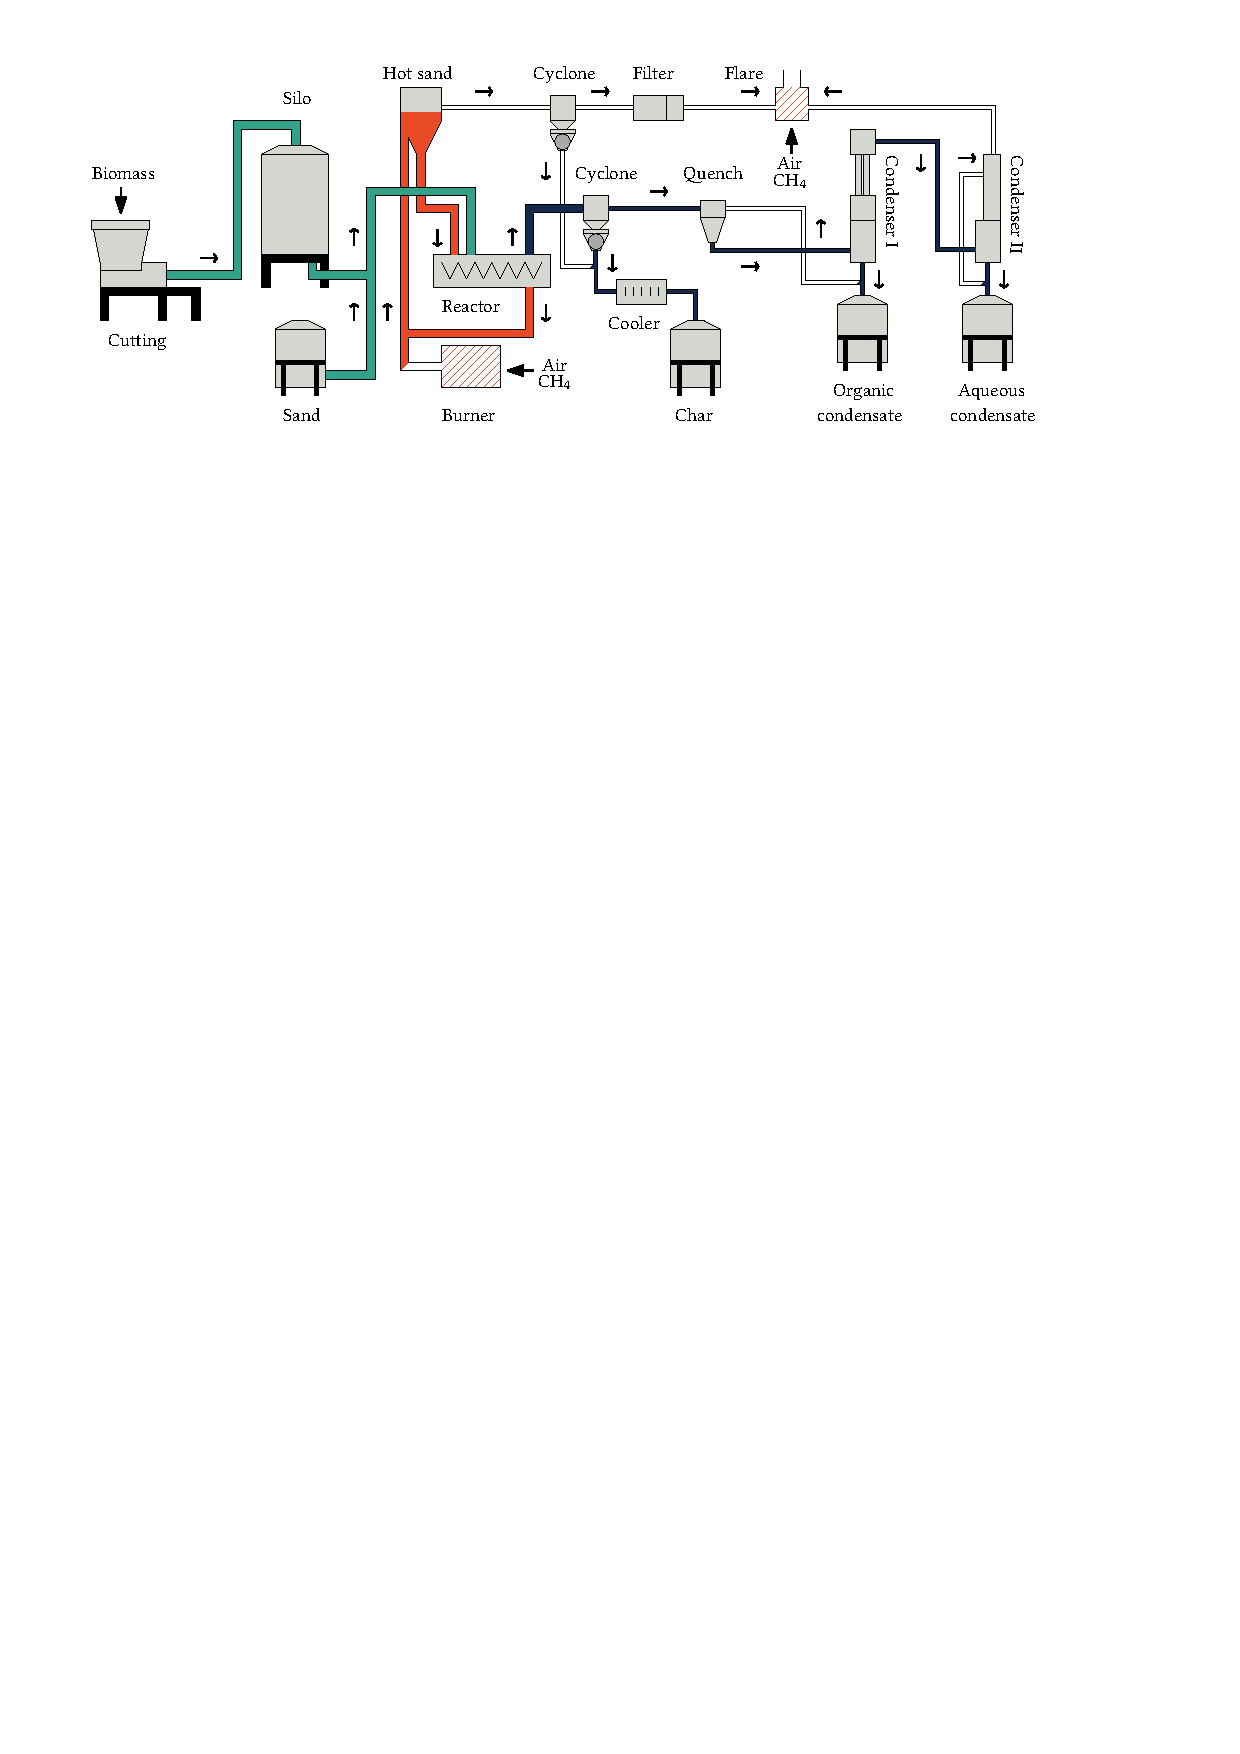
\includegraphics[width=0.95\textwidth]{part1-figures/bioliq_schematics_2-compressed.pdf}\hfill
	\vspace{0.3cm}
	\hfill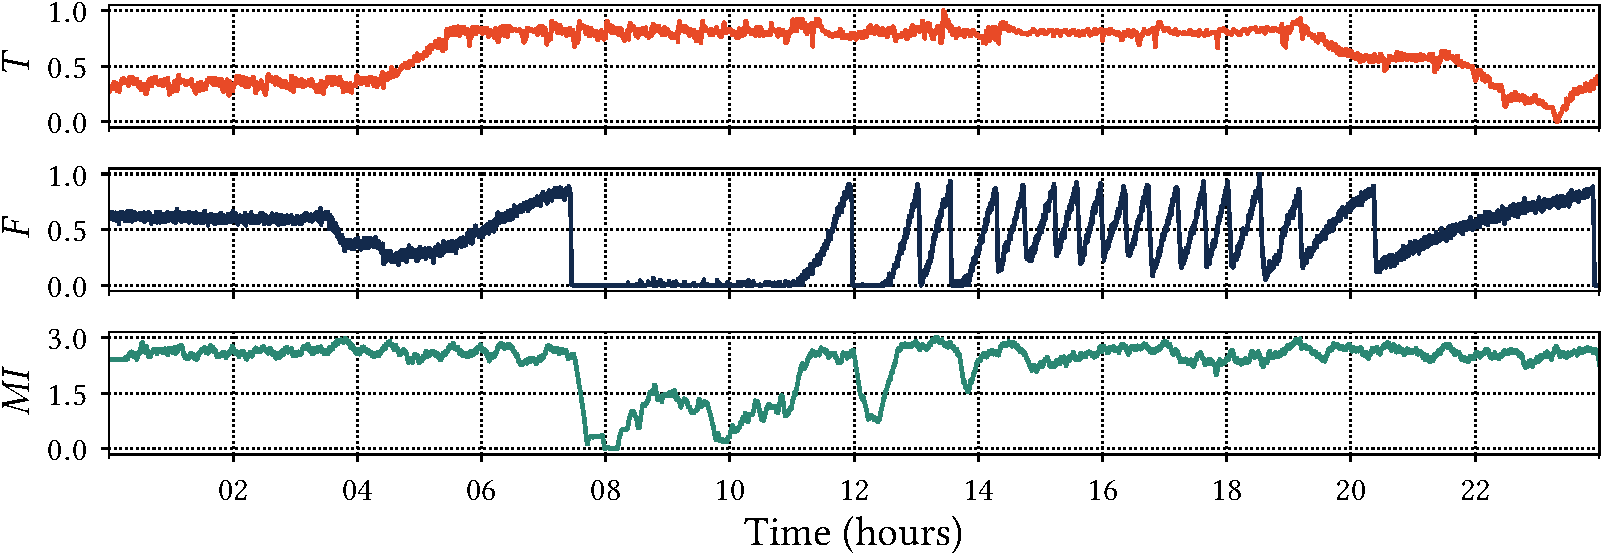
\includegraphics[width=0.95\textwidth]{part1-figures/bioliq_prep_s-crop-compressed.pdf}\hfill
	\caption{Schematics of the \acrshort{Bioliq} fast pyrolysis and monitoring example.}\label{fig:bioliq_schematics}
\end{figure}

\begin{example}[Monitoring at \acrshort{Bioliq}]
	Let us observe a 24-hours measurement period of two sensors at \gls{Bioliq}: $T$ is the temperature in the reactor, and $F$ is the filling level of the flue gas cyclone connected to its output. We report the \gls{MI} between $T$ and $F$ at any time over the last 15 minutes. 
	In the beginning, the reactor heats up to its operational temperature. The material introduced leads to the exhaustion of flue gas, stored temporarily in the cyclone for further processing. The  \gls{MI} between the two streams suddenly drops from 2.5 bits to 0 at 7:45. The cyclone does not seem to operate as it should, i.e., as in the later timespan between 12:00 and 20:00. The data indicates an interruption in production. Such interruptions can become very costly if unnoticed. Thus, the careful monitoring of plant elements is essential, as drifting dependencies might indicate abnormal events \cite{DBLP:journals/tim/Hashemian11}. 
	%See \url{https://www.bioliq.de} for more information about the Bioliq process.
\end{example}
%Note: I am not sure that this is very conclusive at this point 
%We discuss here one possible use case, but the Bioliq plant provides numerous similar examples. The Bioliq plant capture typical use cases from the field of \textit{predictive maintenance}, which represent a primary application of our research.  
%Maybe add a small paragraph saying what the bioliq data is made of. (attributes... etc) and that we will release it. 

\section{Contributions}

The goal of this dissertation is to address the challenges of Data Mining w.r.t. high-dimensionality and streaming data. To this end, we first focus on fundamental problems of Data Mining: estimating dependency and monitoring. Then, we show how our new methods help to address Knowledge Discovery in high-dimensional data streams. We organise our contributions around the three following research questions: 

\begin{itemize}[noitemsep]
	\item \hypertarget{Q1}{\textbf{Q1 (Estimating Dependency):}} The increasing number of dimensions and observations challenge dependency estimation. How to estimate dependency in high-dimensional data streams efficiently and effectively? 
	\item \hypertarget{Q2}{\textbf{Q2 (Monitoring):}} By nature, data streams are infinite and may evolve, so the relationship between variables might change. How can we keep track of the evolution of statistics (e.g., dependency estimates) in streams with high-dimensionality?  
	\item \hypertarget{Q3}{\textbf{Q3 (Knowledge Discovery):}} We see the answer to \hyperlink{Q1}{\textbf{Q1}} and \hyperlink{Q2}{\textbf{Q2}} as fundamental to extract knowledge from high-dimensional streams. Thus, we ask: how to leverage our contributions to mine patterns (e.g., anomalies) in this setting?  
\end{itemize} 

To deal with \hyperlink{Q1}{\textbf{Q1}}, we propose a list of desirable features an estimator must ideally fulfil for high-dimensional data streams. Then, we introduce \gls{MCDE}, a framework that quantifies multivariate dependency as the average statistical discrepancy between marginal and conditional distributions, via Monte Carlo (MC) simulations. \gls{MCDE} handles heterogeneity by leveraging three statistical tests: the Mann-Withney U, the Kolmogorov-Smirnov and the Chi-Squared test. We determine a lower bound for the quality of our estimates, which only depends on the number of MC simulations. Such bound allows users to trade estimation accuracy for a computational advantage. We demonstrate that \gls{MCDE} goes beyond the current state of the art regarding dependency estimation by meeting all the features defined previously. Finally, we show against our real-word use case (\gls{Bioliq}) that \gls{MCDE} can discover useful patterns in high-dimensional data streams. We recently published those results in \cite{DBLP:conf/ssdbm/FoucheB19, DBLP:conf/ssdbm/FoucheBMKB20}. 

Concerning \hyperlink{Q2}{\textbf{Q2}}, we propose to formulate the problem of monitoring statistics in high-dimensional data streams as a \gls{MAB} problem. We find that our setting requires to extend the existing models, and call our extension the \gls{S-MAB}. We propose a new algorithm based on \gls{TS}, with strong theoretical guarantees and excellent empirical performance. Furthermore, we combine our algorithm with \gls{ADWIN}, a state-of-the-art change detector, to deal
with non-static environments. We illustrate the benefits of our contribution using synthetic data, as well as data from our real-world use case. We published our findings in \cite{DBLP:conf/kdd/FoucheKB19}. 

Finally, we address \hyperlink{Q3}{\textbf{Q3}} by exploiting synergies between our previous contributions. We show that, by combining the ideas behind \gls{MCDE} and \gls{S-MAB}, we can facilitate the search for subspaces in data streams. We introduce a new algorithm, \gls{SGMRD}, and show that \gls{SGMRD} leads to state-of-the-art performance for Knowledge Discovery tasks, such as outlier detection. Then, we propose a new method, \gls{kj-NN}, to detect outlying documents within large text corpora. Those contributions are featured here \cite{DBLP:conf/ssdbm/FoucheMGZBH20, DBLP:conf/review/FoucheKB20}.

%All in all, the goal of this dissertation is to establish fundamental tools for knowledge discovery in high-dimensional data streams. We propose efficient methods for estimating and monitoring dependency, which plays a central role in most Data Mining approaches.

\section{Outline}

We structure the rest of this dissertation as follows: 

\begin{itemize}
	\item Chapter \ref{chapter:preliminaries} is a joint introduction to our contributions w.r.t. \hyperlink{Q1}{\textbf{Q1}}, \hyperlink{Q2}{\textbf{Q2}} and \hyperlink{Q3}{\textbf{Q3}}. We introduce a set of desirable features for dependency estimators in high-dimensional data streams and formulate the problem of monitoring in high-dimensional data streams as a \acrfull{MAB} problem. Then, we discuss our applications to Knowledge Discovery in high-dimensional data streams.
	\item Chapter \ref{chapter:relatedwork} presents the related work concerning each of our contributions. 
	\item Part \ref{partII} focuses on \hyperlink{Q1}{\textbf{Q1}}. In Chapter \ref{chapter:MCDE}, we present a new framework for dependency estimation: \acrfull{MCDE}. 
	\item Part \ref{partIII} answers \hyperlink{Q2}{\textbf{Q2}}. Chapter \ref{chapter:S-MAB} introduces the \acrfull{S-MAB} algorithms, our solution to monitor high-dimensional data streams. 
	\item Part \ref{partIV} deals with \hyperlink{Q3}{\textbf{Q3}}. Chapter \ref{chapter:subspacesearch} introduces a general method for Subspace Search in Data Streams, named \acrfull{SGMRD}. Chapter \ref{chapter:textoutlier} presents a new algorithm, \acrfull{kj-NN}, to detect outlying documents within large text corpora.
	\item Part \ref{partV} concludes by summarising the outcome of this dissertation in Chapter \ref{chapter:summary}, while Chapter \ref{chapter:futurework} provides an outlook on future work and research directions.  
\end{itemize}

The content relevant to this dissertation extends beyond the scope of this document. Readers may find complementary information about Bioliq in the literature \cite{pfitzer2016fast} and the official website of the Bioliq project: 
\begin{itemize}
	\item Bioliq: \url{https://www.bioliq.de}
\end{itemize}

Furthermore, we systematically release our source code, data and experiments via open-source platforms, under the GNU Affero General Public License version 3 (\href{https://www.gnu.org/licenses/agpl-3.0.en.html}{AGPLv3}): 

\begin{itemize}
	\item \gls{MCDE}: \url{https://github.com/edouardfouche/MCDE-experiments}; \url{https://github.com/edouardfouche/MCDE}; \url{https://github.com/edouardfouche/MCDE-extended}
	\item \gls{S-MAB}: \url{https://github.com/edouardfouche/S-MAB}
	\item \gls{SGMRD}: \url{https://github.com/edouardfouche/SGMRD} 
	\item \gls{kj-NN}: \url{https://github.com/edouardfouche/MiningTextOutliers} 
\end{itemize}

See also the related entries on the author's website  (\url{https://edouardfouche.com}) and the sources of this document (\url{https://github.com/edouardfouche/phd-thesis}), under the Creative Commons Attribution-ShareAlike 4.0 International License (\href{https://creativecommons.org/licenses/by-sa/4.0/}{CC BY-SA 4.0}).

\chapter{Preliminaries}
\glsresetall
\label{chapter:preliminaries}

This chapter is a joint introduction to our core contributions. % and bases on several publications associated with this dissertation, in particular: \cite{DBLP:conf/ssdbm/FoucheB19, DBLP:conf/ssdbm/FoucheBMKB20, DBLP:conf/kdd/FoucheKB19, DBLP:conf/ssdbm/FoucheMGZBH20, DBLP:conf/review/FocuheKB20}. 
We describe the underlying motivations and the notation for our work. %, organised around our three main topics: Estimating Dependency, Monitoring and Knowledge Discovery.

\section{Estimating Dependency}

\subsection{Motivations}  

The discovery of relationships between attributes is fundamental to many Data Mining applications, e.g., Feature Selection \cite{DBLP:journals/pami/PengLD05}, Clustering \cite{DBLP:conf/sdm/BohmKMNV13} or Outlier Detection \cite{DBLP:conf/icde/KellerMB12}, and it is a prominent topic in the database community \cite{DBLP:journals/tkde/ChenHY96, DBLP:conf/vldb/ZhuS02, DBLP:journals/tkde/HallH03}. 

One typically estimates the strength of a relationship by estimating the `dependence' among the attributes of a subspace. To do so, one often leverages well-known `dependency estimators' such as the Pearson correlation coefficient (also known as \textit{correlation}), or \gls{MI} \cite{DBLP:journals/bstj/Shannon48} as a non-linear counterpart. 

Dependency estimation not only plays a central role in Data Mining -- as we discussed in Section~\ref{sec:centralrole} -- but also delivers useful information per se: knowing the relationship between attributes helps to predict and understand certain outcomes. 

\glsunset{Bioliq}
For instance, knowing that weight and arterial pressure correlate with the odds of contracting certain diseases may guide physicians, when predicting whether a patient will become sick within a year or not. Dependency may also reflect natural physio-chemical relationships, say, between the temperature and pressure of a fluid in a pipe. When dependency changes, it either means that the system's state is transitioning, e.g., the fluid solidifies, or that equipment deteriorates, e.g., there is a leak. Fluctuations of dependency often reflect changes in the stream, i.e., the dependency matrix delivers information about the state of a system. This applies, for example, to the \gls{Bioliq} plant (Figure \ref{fig:bioliq_schematics}). 

However, concerning real-world settings, dependency estimation remains mostly unaddressed: data often comes as an open-ended, ever-evolving stream of sensor signals. The signals can be noisy, redundant or generated at a varying speed. In this setting, the timely detection of changes in the stream is crucial; the early discovery of anomalies can, say, facilitate predictive maintenance and yield tremendous cost savings.

Also, most dependency estimators only deal with numerical data, while the stream often consists of measurements or indicators of various types, e.g., numerical, ordinal, or categorical observations. Such data sources are known as \textit{Heterogeneous Data Streams} \cite{DBLP:conf/icdm/YangZ06}. In Section \ref{challenges:datastreams}, we reviewed the constraints associated with data streams. Naturally, addressing those constraints is a prerequisite for any algorithm operating on streams. 
%Knowledge discovery in H-DS is known as one of the most challenging problems in Data Mining  \cite{DBLP:journals/cim/DitzlerRAP15}, as we discussed previously.  

With this in mind, and orthogonally to the constraints of the streaming setting, modern dependency estimators also have their own set of requirements -- or desirable features -- that they ideally must fulfil. We describe those requirements hereafter. 
%\enlargethispage{\baselineskip}

\subsection{Requirements}

Based on our observation of the current state of the art, our first contribution is to establish the following set of requirements, that any dependency estimator must ideally satisfy:

\begin{itemize}[noitemsep]
	\item \hypertarget{R1}{\textbf{Multivariate (R1):}} Bivariate measures only apply to two entities (i.e., variables, vectors). Estimating the dependency between more than two entities is useful as well, but existing attempts to generalise bivariate measures lack efficiency or effectiveness. %\cite{DBLP:conf/aaai/WangRNBMX17}. 
	
	\item \hypertarget{R2}{\textbf{General-purpose (R2):}} Estimators should not restrict to specific types of dependencies. Otherwise, they may miss relevant attribute relationships. Existing multivariate estimators are typically limited to, say, monotonous or functional dependencies. 
	
	\item \hypertarget{R3}{\textbf{Intuitive (R3):}} A method is intuitive if its parameters are easy to set, i.e., users understand their impact on the estimation. 
	Existing solutions tend to have unintuitive parameters, and the suggestion of `good' parameter values happens (or does not happen) at the discretion of the inventors. 
	
	\item \hypertarget{R4}{\textbf{Non-parametric (R4):}} Since real data can exhibit virtually any kind of distribution, it is not reasonable to use measures relying on parametric assumptions. The risk is to miss relevant effects systematically.
	
	\item \hypertarget{R5}{\textbf{Interpretable (R5):}} The results of dependency estimators should be interpretable. In particular, the returned estimate should have a maximum and a minimum, so that one can interpret and compare two given estimates.
	
	\item \hypertarget{R6}{\textbf{Sensitive (R6):}} Dependency estimation is not only about detecting the existence of a relationship, but also about quantifying its strength. Data points generally are observations sampled from a potentially noisy process. The same dependency should get a higher score when observed with more observations, as the size of the observed effect -- the `effect size' -- is larger. 
	
	\item \hypertarget{R7}{\textbf{Robust (R7):}} Real-world data may be of poor quality. Measuring devices often have limited precision, so that values are rounded or trimmed, leading to points with the same values. It is also common to discretise attributes, for a more compact representation. Such artefacts can have a negative influence on the estimation. Thus, estimators need to be robust against duplicates and imprecision. 
\end{itemize}

To the best of our knowledge, any existing solution only fulfils some of those requirements at best.
For example, the Pearson correlation coefficient is parametric (\hyperlink{R4}{\textbf{R4}}), targets at linear dependencies (\hyperlink{R2}{\textbf{R2}}) and is only applicable to numerical data (\hyperlink{C5}{\textbf{C5}}). 
%Note: Maybe we could talk about alternative requirement definitions

There exist alternative criteria to compare dependency estimators. For example, \cite{doi:10.1007/BF02024507} propose a set of rules that dependency estimators should satisfy. However, there is no standard benchmark and, for most estimators, whether they meet those rules or not is unknown. \cite{Reshef1518} propose to evaluate measures against a notion of `equitability'. However, there is so far no commonly accepted formalisation of this notion \cite{Kinney2013, MurrellE2160}. In contrast, we introduce a set of pragmatic characteristics, focusing on the real-world requirements of dependency estimators in high-dimensional data streams.

In this dissertation, we propose a framework, \gls{MCDE}, which features these characteristics and compare \gls{MCDE} via systematic experiments with the existing competitors. In the next section, we introduce our notation. 

\subsection{Notation}
\label{sec:mcdenotations}

A data stream is a set of attributes $\gls{D}=\{s_1, \dots, s_{|\gls{D}|}\}$ and an open list of observations $\gls{B} = (\vec{\gls{x}}_{1}, \vec{\gls{x}}_{2}, \dots)$, where $\vec{\gls{x}}_i = \langle x_{ij} \rangle_{j \in \{1, \dots, |\gls{D}|\}}$ is a vector of values with $|\gls{D}|$ attributes, and we see an attribute $\gls{s_i} = (x_{1i},x_{2i},\dots)$, with $i \in \{1,\dots,|\gls{D}|\}$, as an open list of values. %Note that we use the terms attribute, dimension and variable interchangeably. 

Since the stream is virtually infinite, we use the sliding window model: At any time $\gls{t} > 1$, we only keep the $\gls{w}$ latest observations, $\gls{W_t} = \left(\vec{\gls{x}}_{\gls{t}-\gls{w}+1}, \dots, \vec{\gls{x}}_{\gls{t}} \right)$. We assume, without loss of generality, that observations arrive at equidistant time steps. Note that one could easily adapt our methods to accommodate other summarisation techniques, such as the landmark window or reservoir sampling \cite{DBLP:journals/pai/Gama12}. %Note: Maybe emphasize why is it so
Figure \ref{fig:slidingwindow} illustrates our notation. 

\begin{figure}
	\centering
	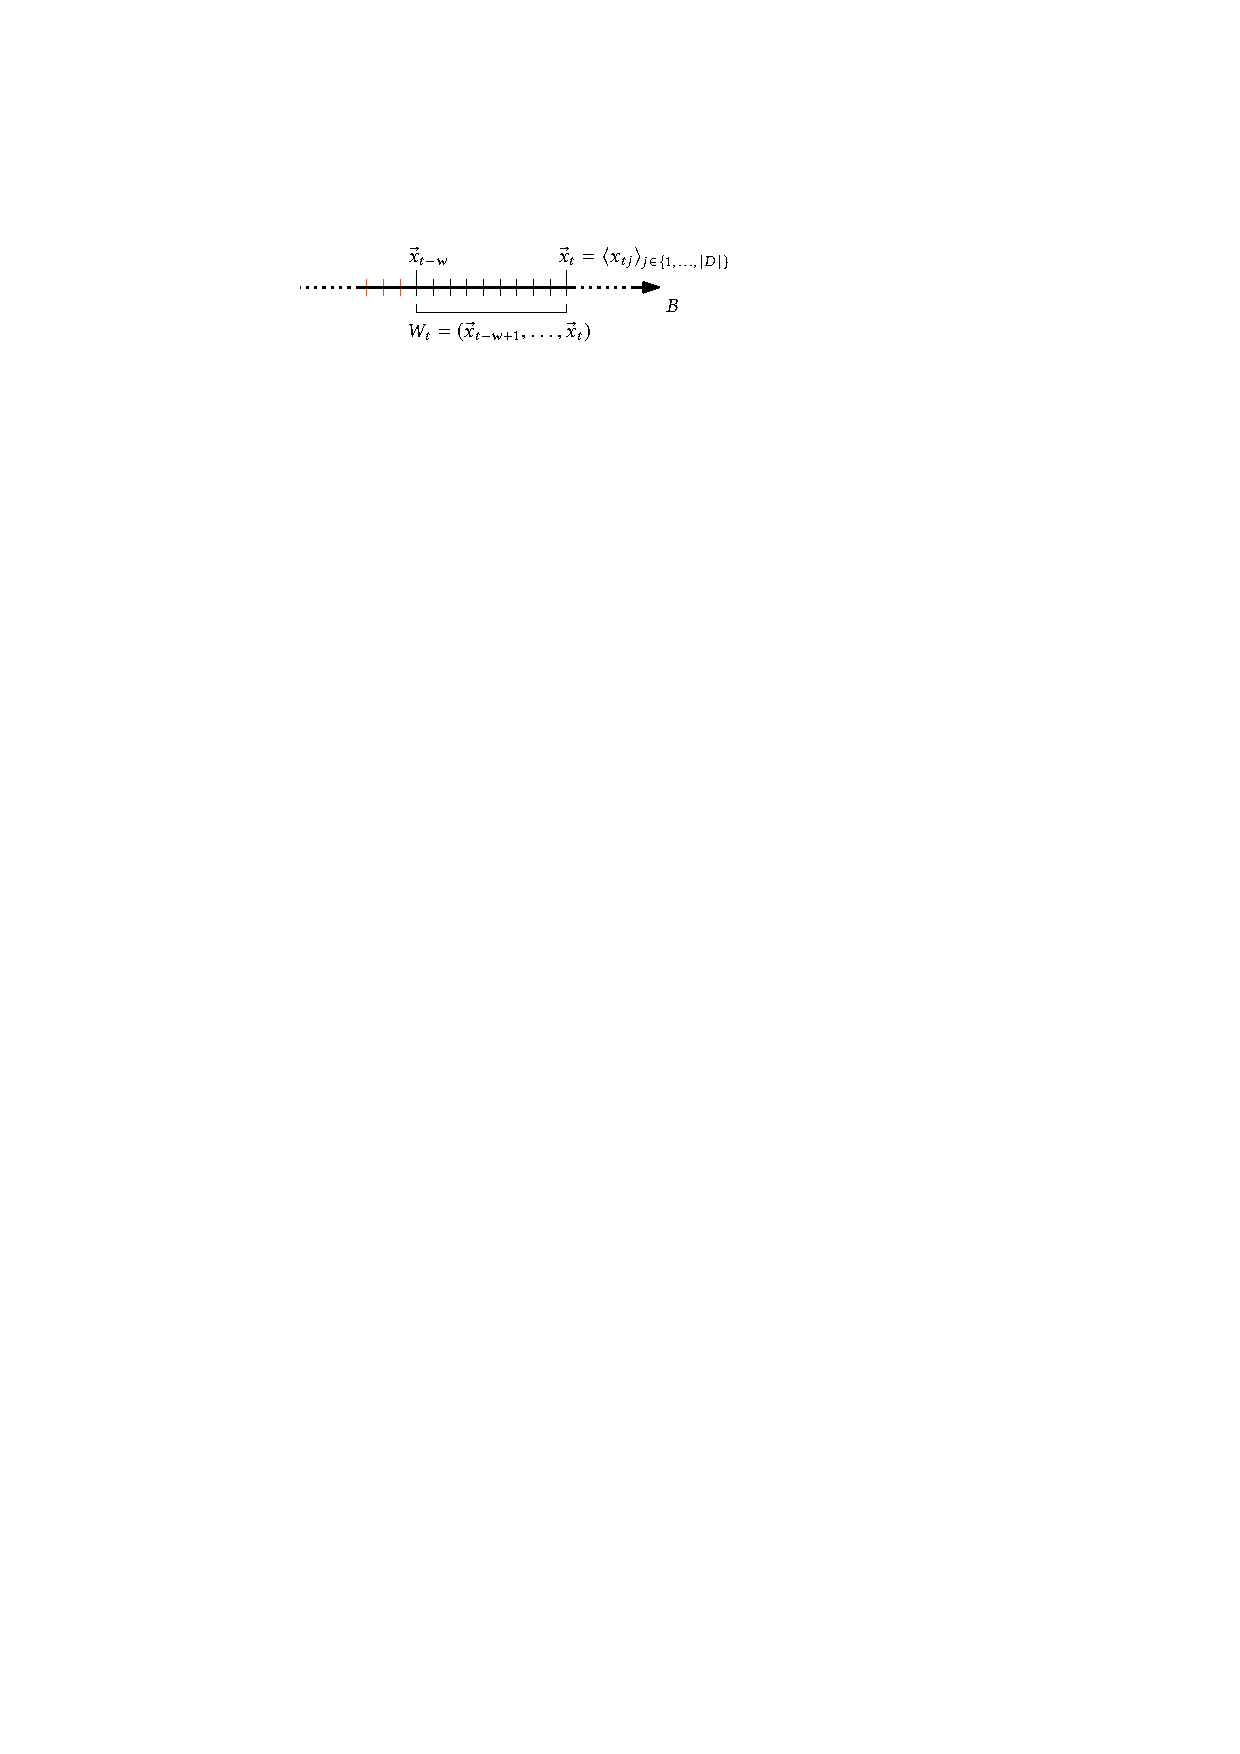
\includegraphics[width=0.6\textwidth]{part1-figures/slidingwindow-compressed.pdf}
	\caption{The sliding window contains the $\gls{w}$ latest observations (here, $\gls{w}=10$).}\label{fig:slidingwindow}
\end{figure}

We call a subspace $\gls{S}$ a projection of the window $\gls{W_t}$ on $|\gls{S}|$ attributes, with $\gls{S} \subseteq \gls{D}$ and $|\gls{S}| \leq |\gls{D}|$. 
We treat an attribute $\gls{s_i} \in \gls{D}$ as a random variable $\gls{X_{s_i}}$.  To address \textit{heterogeneity}, we also make the distinction between numerical, ordinal and categorical attributes:
\begin{itemize}[noitemsep]
	\item We say that $\gls{s_i}$ is of numerical type ($\gls{s_i} \in \mathit{\gls{Num}}$) 
	if one can see $\gls{X_{s_i}}$ as a continuous variable on a given interval. 
	\item We say that $\gls{s_i}$ is of ordinal type ($\gls{s_i} \in \mathit{\gls{Ord}}$) if one can see  $\gls{X_{s_i}}$ as a discrete variable, i.e., it can take a finite number of ordered values.
	\item We say that $\gls{s_i}$ is of categorical type ($\gls{s_i} \in \mathit{\gls{Cat}}$) if  one can see $\gls{X_{s_i}}$ as a categorical variable, with a fixed amount of nominal categories.
\end{itemize}

Naturally, knowing whether a given attribute is numerical, ordinal or categorical requires domain knowledge. Typically, ordinal attributes have many tying values, while values from a numerical attribute are unique, given enough precision. On the other hand, values from categorical attributes might not be numeric and do not have any meaningfully ordering. 

Then, $\gls{p(X)}$ is the joint probability distribution function (\textit{pdf}) of a random vector $\gls{X} = \left \langle \gls{X_{s_i}}\right \rangle  _{\gls{s_i} \in \gls{S}}$, and $\hat{p}(X)$ denotes the empirical estimation of this distribution. 
We use $\gls{p_{s_{i}}(X)}$ and $\hat{p}_{s_{i}}(X)$ for the marginal \textit{pdf} and its estimation for each variable $\gls{s_i}$.
$\gls{P}(\gls{S})$ is the power set of $\gls{S}$, i.e., the set of all attribute subsets. 
For any subset $S' \in \gls{P}(\gls{S})$, its random vector is $\gls{X}_{S'}= \left \langle \gls{X_{s_i}}\right \rangle _{\gls{s_i} \in S'}$ and its complement $\overline{X_{S'}} = X_{\gls{S}  \setminus S'} = \left \langle \gls{X_{s_i}}\right \rangle _{\gls{s_i} \in \gls{S} \setminus S'}$. 
In our algorithms, `$\oplus$' and `$\wedge$' stand for concatenation and element-wise logical conjunction. 

Dependency estimation determines to which extent a relationship differs from randomness. In this spirit, \gls{MCDE} quantifies a dependency, i.e., a degree of independence violation, based on marginal and conditional distributions. In Part \ref{partII}, we extensively describe \gls{MCDE}. 

Nonetheless, \gls{MCDE} only estimates the dependency within a given subspace. In the next section, we abstract from the underlying dependency estimator and consider the problem of monitoring numerous estimates in high-dimensional data streams. 

\section{Monitoring}

\subsection{Motivations} 
%Note: According to S. Muthukrishnan et al. Data streams: Algorithms and applications, I am using the time-series model (as opposed to additive and turnstile) (source: Boidol)

Monitoring, i.e., the real-time computation of statistics (such as dependency estimates), is crucial for Knowledge Discovery in data streams. Transient statistics may reveal the
current state of manufacturing machines or the ongoing behaviour of financial markets. 

However, monitoring is computationally demanding, especially when the number of dimensions and the rate of incoming data increase (cf. Sections \ref{challenges:highdimensionality} and \ref{challenges:datastreams}). %First, the number of pairs/subspaces grows quadratically/exponentially with the number of variables (cf. Section \ref{challenges:highdimensionality}). Second, a stream may evolve in unforeseen ways, i.e., each statistics become a time-dependent concept (cf. Section \ref{challenges:datastreams}). 
In this setting, recomputing the statistics at every time step does not scale. Thus, stream statistics monitoring -- for say, high-frequency trading or the monitoring of large factories -- is impractical with current methods. At the same time, it can be advantageous. Think for example of monitoring dependency in the \gls{Bioliq} plant: 

\begin{example}[Dependency Monitoring]
	\label{bandit:runningexample}
	Dependency often results from physical relationships between, say, the temperature and pressure of a fluid. 
%	When dependency changes, this means that the system is transitioning into another state, e.g., the fluid solidifies, or that equipment deteriorates or fails, e.g., there is a leak.
	When monitoring the pyrolysis process at \gls{Bioliq}, it is useful to maintain an overview of dependencies to keep operation costs down.  
	However, continuously updating the complete dependency matrix is impractical with current methods since the data is typically high-dimensional and ever-evolving. 
\end{example}

From a practical point of view, all statistics are not equally interesting. For example, for Knowledge Discovery, one is often interested in high dependency. Our idea is to update only a few elements of the matrix, based on a notion of `utility', e.g., high dependency values. The system must minimise the cost of monitoring while maximising the total utility. %, in a possibly non-static environment. 
In other words, the system faces a trade-off between exploitation and exploration: Should the system keep updating estimates known to deliver large utility (gain) or use resources to update other estimates, for which the potential utility is not yet well-known? 

%Put differently, one idea is to periodically update only a portion of the statistics over time, following a strategy that is learned online, i.e., the monitoring system decides which estimate to update. Based on the outcome, the system adjusts its strategy for future decisions. 

In this dissertation, we see the problem of monitoring as a generalisation of the \gls{MAB} problem. The \gls{MAB} problem captures the dilemma between exploration and exploitation in sequential decision-making. At every time step, a forecaster selects a set of arms and observes a reward from each arm. The name of the \gls{MAB} problem finds its origin in the typical trade-off a gambler faces in a casino: given a set of slot machines (see Figure \ref{fig:MAB}), a.k.a.\ `one-armed bandits', which machine should the gambler play to maximise their expected gains? Should they try different machines (exploration) or keep playing the machine that they believe to be the best so far (exploitation)?   

\begin{figure}
	\centering
	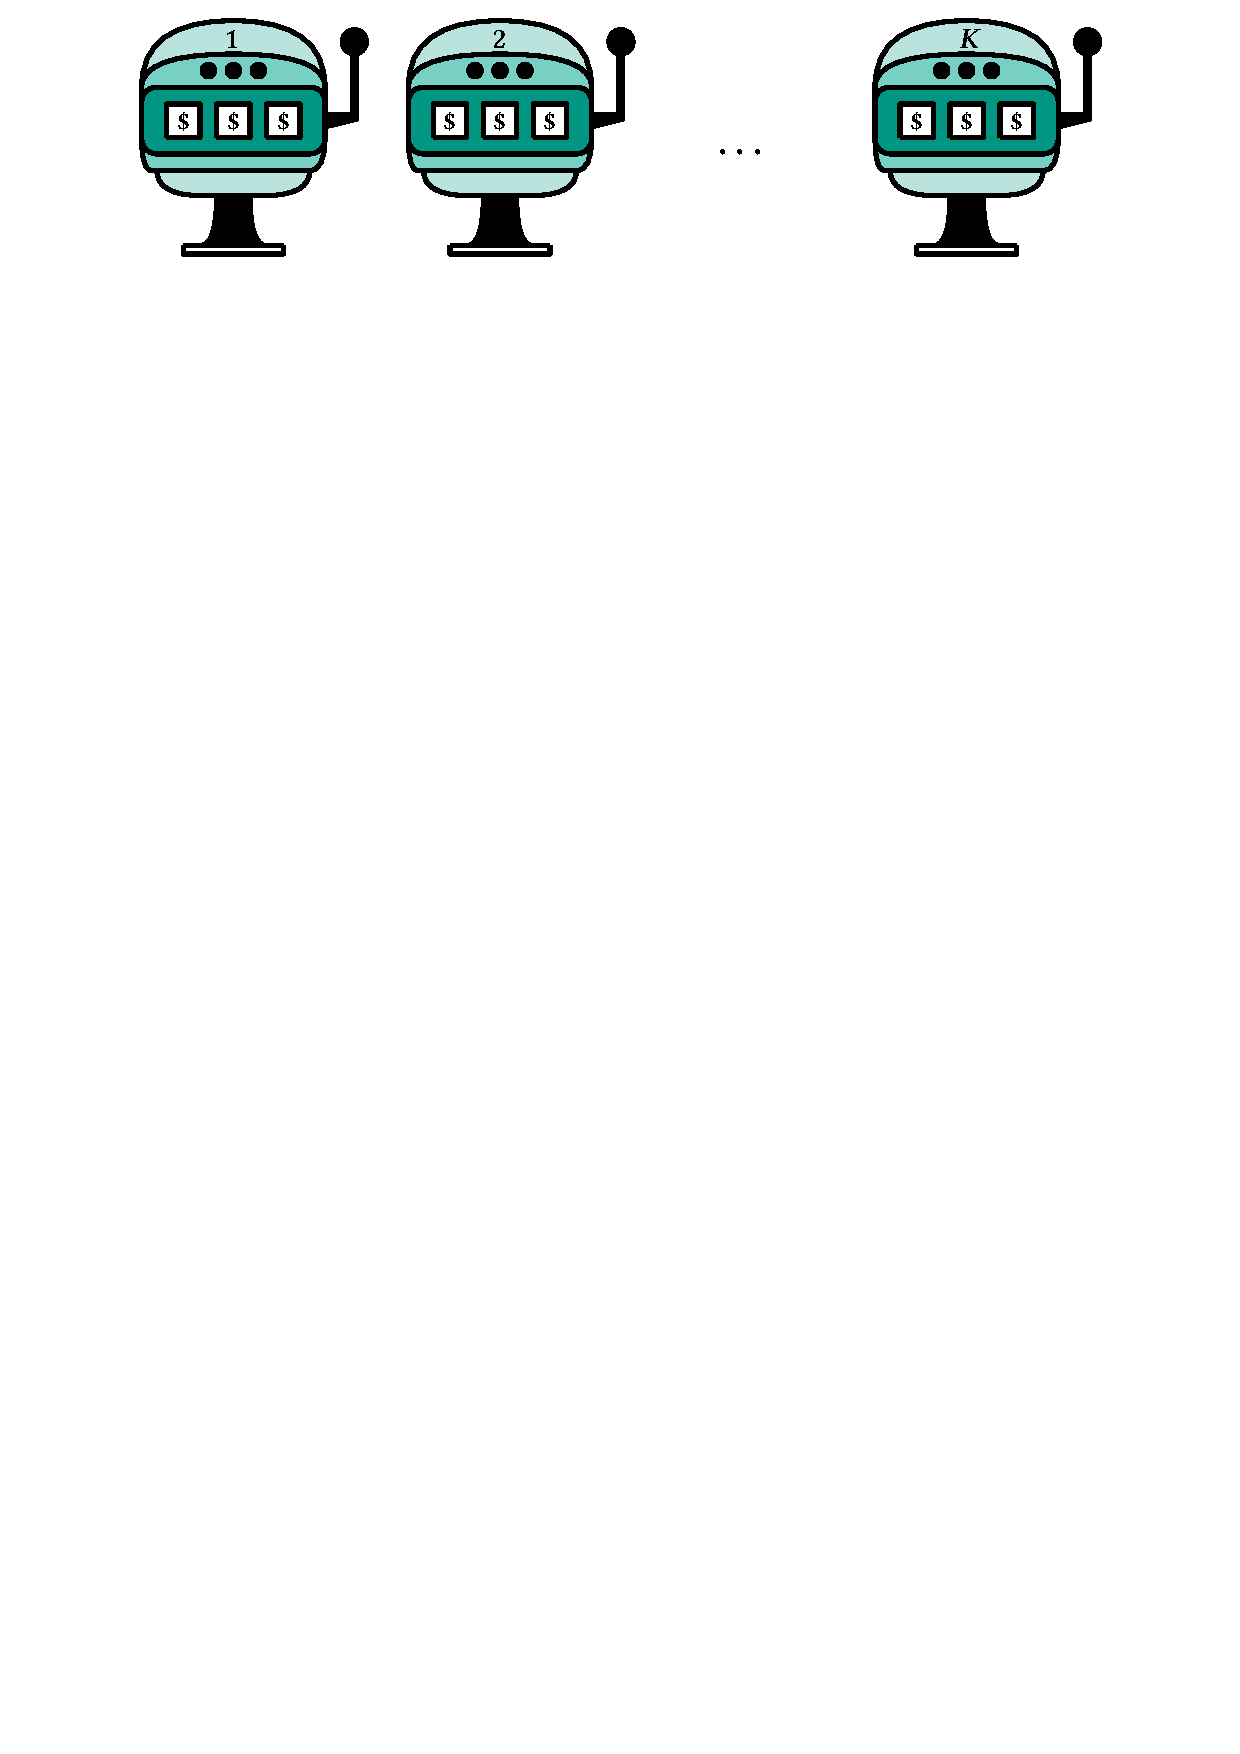
\includegraphics[width=0.70\textwidth]{part1-figures/bandit_1tok-compressed.pdf}
	\caption{The \acrshort{MAB} problem with $\gls{K}$ arms (one-armed bandits).}
	\label{fig:MAB}
\end{figure} 

However, the existing \gls{MAB} formulations do not quite match our problem, as we will see. In what follows, we propose to cast data stream monitoring as a new bandit problem, that we call the \gls{S-MAB}. 

\subsection{Monitoring as a Bandit Problem} 

In the classical \gls{MAB} problem, a forecaster must choose one of $\gls{K}$ arms at each round, and playing it yields a reward. Their goal is to maximise the cumulative reward over time. In a variant of the problem, known as the \gls{MP-MAB} \cite{1104491,DBLP:conf/icml/KomiyamaHN15}, the forecaster must choose $\gls{L}$ distinct arms per round, where $\gls{L}$ is an exogenous parameter. However, while it is relevant for some applications (e.g., web content optimisation), adequately setting $\gls{L}$ is not easy when monitoring streams. %, as well as further applications. %While in some applications, such as web content optimisation
%, $L$ is given, when monitoring data streams, an appropriate value of $L$ is not obvious. 

Thus, we consider a new variant of the \gls{MP-MAB} where the forecaster not only must choose the best arms but also must `scale' $\gls{L}$, i.e., change the number of plays, to maximise the rewards and minimise the costs. % at any time. 
By doing so, the forecaster controls the efficiency of playing. We name this setting the \acrfull{S-MAB} problem.

Think of a new casino game, which we call the `blind roulette': the player places bets on distinct numbers, and each number has an independent but unknown probability of being drawn. Bets correspond to a fixed amount, e.g., one can only bet $1$\$ on a number or nothing. 
In each round, the player must decide how many bets to place, and on which numbers. 
The casino then reveals to the player which ones of their bets were successful and pays the corresponding reward. To make the game more challenging, the casino may sometimes change the underlying probability of each number without notice.  

While placing a few but confident bets may seem to be an economically efficient option, the absolute gain at the end of the day will not be significant. 
On the other hand, placing many bets may not be a good strategy, as many numbers typically have a low chance to be drawn. 
To maximise their gain, the player must place as many bets as possible, as long as their expected gain is higher than the amount bet. 
Whenever the probabilities change, the player needs to adapt their behaviour; otherwise, they may lose most of their bets and experience much regret w.r.t.\ an optimal (but unknown) strategy.

This game matches not only dependency monitoring (cf. Example \ref{bandit:runningexample}) but also many other real-world applications, such as the placement of online advertisements or the investment in financial portfolios. The \gls{S-MAB} problem introduces a new trade-off: one wants to maximise the reward, but at the same time minimise the cost of each round/observation. The problem consists of the following challenges: 

\begin{itemize}[noitemsep]
	\item \hypertarget{*1}{\textbf{*1: Top-arms Identification.}} To maximise the reward from $\gls{L}$ plays, one needs to find the $\gls{L}$ arms with the highest expected reward; This is the traditional exploration-exploitation dilemma known from the \gls{MP-MAB} problem.
	
	\item \hypertarget{*2}{\textbf{*2: Scale Decision.}} One should not play more arms than necessary: playing many arms leads to high costs, but playing only a few arms leads to low rewards. One should set $\gls{L}$ to control the efficiency, i.e., the ratio of the rewards to the costs.
	
	\item \hypertarget{*3}{\textbf{*3: Change Adaptation.}} The environment can either be static or non-static. In the second case, one needs to `forget' prior knowledge whenever a change occurs. Forgetting that is too aggressive or too conservative leads to suboptimal results.
\end{itemize}
In the next section, we formalise the \gls{S-MAB} problem considering those challenges\footnote{See also \url{https://youtu.be/wVogcI3fr7Q} for a 3-minute introduction to this problem.}. We use the most common notation from the bandit literature, e.g., as in \cite{DBLP:journals/ftml/BubeckC12}. 

\subsection{Problem Definition}
\label{section:notationsbandits}

Let there be $\gls{K}$ arms. We associate each arm $i \in [\gls{K}]  = \left\{1,\dots,\gls{K}\right\}$ with an unknown probability distribution $v_i$ with mean $\gls{mu_i}$. 
At each round $\gls{t} = 1, \dots, \gls{T}$, the forecaster selects arms $\gls{I(t)} \subset [\gls{K}]$, then receives a reward vector $\gls{X(t)}$. 
$\gls{L}_{\gls{t}} \le \gls{K}$ is the number of these arms.
The rewards $\gls{X_i(t)} \in \gls{X(t)}$ of each arm $i$ are i.i.d.\ samples from $v_i$. We make the classical assumption from bandit analysis that the rewards $\gls{X_i(t)}$ are $0$ or $1$, i.e., the distribution of rewards from arm $i \in [\gls{K}]$ follows a Bernoulli distribution with mean $\gls{mu_i}$. 
Selecting an arm $i \in [\gls{K}]$ leads to a unit cost $1$, where cost and reward do not need to have the same unit. Note that it is not very difficult to generalise our results to other reward distributions, as long as they are bounded. 

Let $\gls{N_i(t)}$ and $\gls{S_i(t)}$ be the number of draws of arm $i$ and the sum of the rewards obtained from it respectively before round $t$. Let $\hat{\mu}_i(t) = \gls{S_i(t)}/\gls{N_i(t)}$ be the empirical estimation of $\gls{mu_i}$ at time $\gls{t}$. 
The forecaster is interested in maximising the sum of the rewards over arms drawn, under the constraint that the sum of the rewards must be greater than the sum of the costs by an efficiency factor $\gls{eta^*}$. The parameter $\gls{eta^*} \in [0,1]$ controls the trade-off between the cost of playing and the reward obtained, which is application-dependent. 

Let us think of our `blind roulette' metaphor and assume that, whenever a bet is successful, the casino awards the double of the bet. Then, for positive expectations, the player must set $\gls{eta^*} > 0.5$ and control $\eta_t$, the admitted cost per arm, to be higher than $\gls{eta^*}$. Thus, at each step $\gls{t}$, the forecaster is facing the following constrained optimisation problem: 
\begin{equation}
\underset{\gls{I(t)} \subset [\gls{K}]}{\max} \sum_{i \in \gls{I(t)}} \gls{S_i(t)} \quad s.t. \quad \eta_{\gls{t}} = \frac{\sum_{i \in \gls{I(t)}} \gls{mu_i}}{\gls{L}_{\gls{t}}}  > \gls{eta^*} 
\label{eq1}
\end{equation} 
The difficulty here is that the forecaster does not know $\gls{mu_i}$, but only has access to an estimate $\hat{\mu}_i$ from previous observations. 

$\sum_{i \in \gls{I(t)}} \gls{S_i(t)} $ is maximised when the forecaster chooses the arms with the highest expectation $\gls{mu_i}$. 
For simplicity, we assume that all arms have distinct expectations (i.e., $\gls{mu_i} \neq \mu_j, \forall i \neq j$) and we assume without loss of generality that $\mu_1 > \mu_2 > \dots > \mu_{\gls{K}}$, and thus $[\gls{L}_{\gls{t}}]$ is the top-$\gls{L}_{\gls{t}}$ arms. Under the assumption that the forecaster always chooses $[\gls{L}_{\gls{t}}]$, the value of $\eta_{\gls{t}}$ is only determined by $\gls{L}_{\gls{t}}$, i.e., Eq. \eqref{eq1} is equivalent to finding the optimal number of plays $\gls{L^*}$:
\begin{equation} \label{eq2}
\gls{L^*} = \underset{{1 \leq \gls{L} \leq \gls{K}}}{\max}{\gls{L}} \quad s.t. \quad \frac{\sum_{i=1}^{\gls{L}} \gls{mu_i}}{\gls{L}} > \gls{eta^*}
\end{equation}
Thus, the correct identification of the top-$\gls{L}_{\gls{t}}$ arms (\hyperlink{*1}{\textbf{*1}}) is sine qua non to find the optimal number of plays $\gls{L^*}$ (\hyperlink{*2}{\textbf{*2}}).
Next, in non-static environments, the expected rewards may change, i.e., $\gls{mu_i}: \gls{t} \mapsto [0,1]$ becomes a function of $\gls{t}$, as does $\gls{L^*}$. 
So the forecaster must adapt its estimation $\hat{\mu}_i$ (\hyperlink{*3}{\textbf{*2}}) to correctly select the arms with the highest reward, i.e., it needs to discard outdated observations. 

In Part \ref{partIII}, we present algorithms that solve the \gls{S-MAB} problem and those challenges. Using our contribution, one can monitor dependency in data streams very efficiently. In the next section, we start to reflect on the implications of those contributions w.r.t.\ Knowledge Discovery in high-dimensional data streams. 

\section{Knowledge Discovery}

Part \ref{partIV} shows the impact of our contributions towards a higher-level goal: Knowledge Discovery in high-dimensional data streams. Chapter \ref{chapter:subspacesearch} shows that combining our contributions from Part \ref{partII} and \ref{partIII}, namely \gls{MCDE} and \gls{S-MAB}, helps to transfer the task of subspace search to the streaming setting. We show that the efficient monitoring of subspaces of interest helps with outlier detection in high-dimensional data streams. Then, we deal in Chapter  \ref{chapter:textoutlier} with a real-world use case: the discovery of text outliers from large text corpora and propose a new method to detect such outliers. 

\subsection{Subspace Search in Data Streams}
\label{prelim:subspacesearch}

Analysing high-dimensional data is notoriously difficult (cf. Section \ref{challenges:highdimensionality}). As we discussed in Section \ref{sec:centralrole}, a fundamental task of Data Mining is to quantify the dependence between attributes. %This information helps to understand the data and often improves the result of subsequent Data Mining tasks. 
With this in mind, researchers have proposed \textit{subspace search} methods, mainly for static data, to find interesting low-dimensional projections. Such projections tend to much structure, i.e., high dependence among their dimensions. 
Subspace search is state-of-the-art to deal with data of high dimensionality and has numerous applications, including Exploratory Data Mining \cite{DBLP:journals/sigkdd/AssentKMS07, DBLP:conf/ieeevast/TatuMFBSSK12}, outlier detection \cite{DBLP:conf/icde/ZhangGW08, DBLP:conf/icde/KellerMB12,  DBLP:journals/ijdsa/TrittenbachB19}% vanea2012instant,
, or clustering \cite{DBLP:conf/sigmod/ProcopiucJAM02, DBLP:conf/pkdd/KailingKKW03, DBLP:conf/icdm/BaumgartnerPKKK04, DBLP:conf/cikm/ParkL07, DBLP:conf/icdm/ZhangLW07}.  %Some contributions \cite{DBLP:conf/aaai/WangRNBMX17, DBLP:conf/sdm/BohmKMNV13, DBLP:conf/cikm/KellerMWB13} explicitly address both clustering and outlier detection with the same subspace search approach. 

One can see subspace search as an ensemble \textit{feature selection} method \cite{DBLP:journals/jmlr/GuyonE03}, as the goal is to find several projections (subspaces), not just one. 
The underlying assumption of subspace search is that patterns (e.g., outliers, clusters) may hide in various subspaces \cite{DBLP:books/sp/Aggarwal2013}, and that, when restricting the search to a single subspace, one may miss some patterns. 
In a nutshell, existing subspace search methods consist of two building blocks: 

(1) A \textit{quality measure} to quantify the `interestingness' of a subspace, i.e., the potential to reveal patterns. Intuitively, subspaces with `structure' are more likely to contain outliers or clusters \cite{DBLP:phd/dnb/Keller15}. That measure often is a multivariate measure of dependence. 

(2) A \textit{search scheme} to explore the set of subspaces. Since this set grows exponentially with dimensionality, inspecting every subspace is not possible, and the search typically is a heuristic, i.e., a trade-off between completeness of the search and result quality.

These two items tend to be specific for a given Data Mining algorithm, e.g., a certain clustering method. 
The search then is helpful for this particular algorithm, but does not generalise beyond \cite{DBLP:conf/ieeevast/TatuMFBSSK12}. Next, existing approaches for subspace search tend to assume that the data is static. 
A straightforward generalisation to streams -- i.e., repeating the search periodically -- is computationally expensive and limited by the speed of new observations arriving. 

In Chapter \ref{chapter:subspacesearch}, we exploit synergies between our contributions \cite{DBLP:conf/ssdbm/FoucheB19, DBLP:conf/kdd/FoucheKB19, DBLP:conf/ssdbm/FoucheBMKB20} to facilitate subspace search in streams by fulfilling the constraints of this setting (see Section \ref{challenges:datastreams}). %Our algorithm, \gls{SGMRD}, facilitate subspace search for streams. 
The core idea of our method, \gls{SGMRD}, is to maintain a set of high-quality subspaces over time, by updating subspace-search results continuously. We show that it is advantageous to detect patterns (e.g., outliers) in high-dimensional data streams, and that existing approaches are much less efficient. To describe our approach, we use the same notation as in Section \ref{sec:mcdenotations}. 

%In the next section, we treat a more specific problem: The detection of outlying documents from large text corpora. 

\subsection{Mining Text Outliers}
\label{sec:textoutlierprelim}

\subsubsection{Motivations}

Recent technological developments have led to an ever-growing number of applications producing, sharing and managing text data. Document repositories, such as email accounts, digital libraries or medical archives, have grown so large that it is now a necessity to classify elements into categories, e.g., folders. 

This is far from trivial, as text corpora tend to be highly multi-modal, i.e., there are many classes/folders. 
Documents also may have ambiguous semantics or more than one semantic focus, so that they do not perfectly fit into just one class.
%EF: This introduces "Challenge 1: Multi-Modality"

Humans can order content to some extent and routinely do so: Users organise their emails into folders, authors classify their contributions into existing taxonomies, and physicians issue diagnoses as part of their duties. 
However, human classification is inherently sloppy and unreliable. %prone to errors. 
Humans may classify an email into an inadequate folder, assign scientific papers to the wrong field, or -- even more critical -- issue a wrong diagnosis. 
%EF: This introduces Type M (missclassification)

Sometimes one may not even notice these errors because the correct class is unknown. 
For instance, an email does not fit into any existing folder, a paper belongs to an emerging field, or a physician observes a new disease.  %EF: This introduces Type O (out-of-distribution)

\begin{figure}
	\centering
	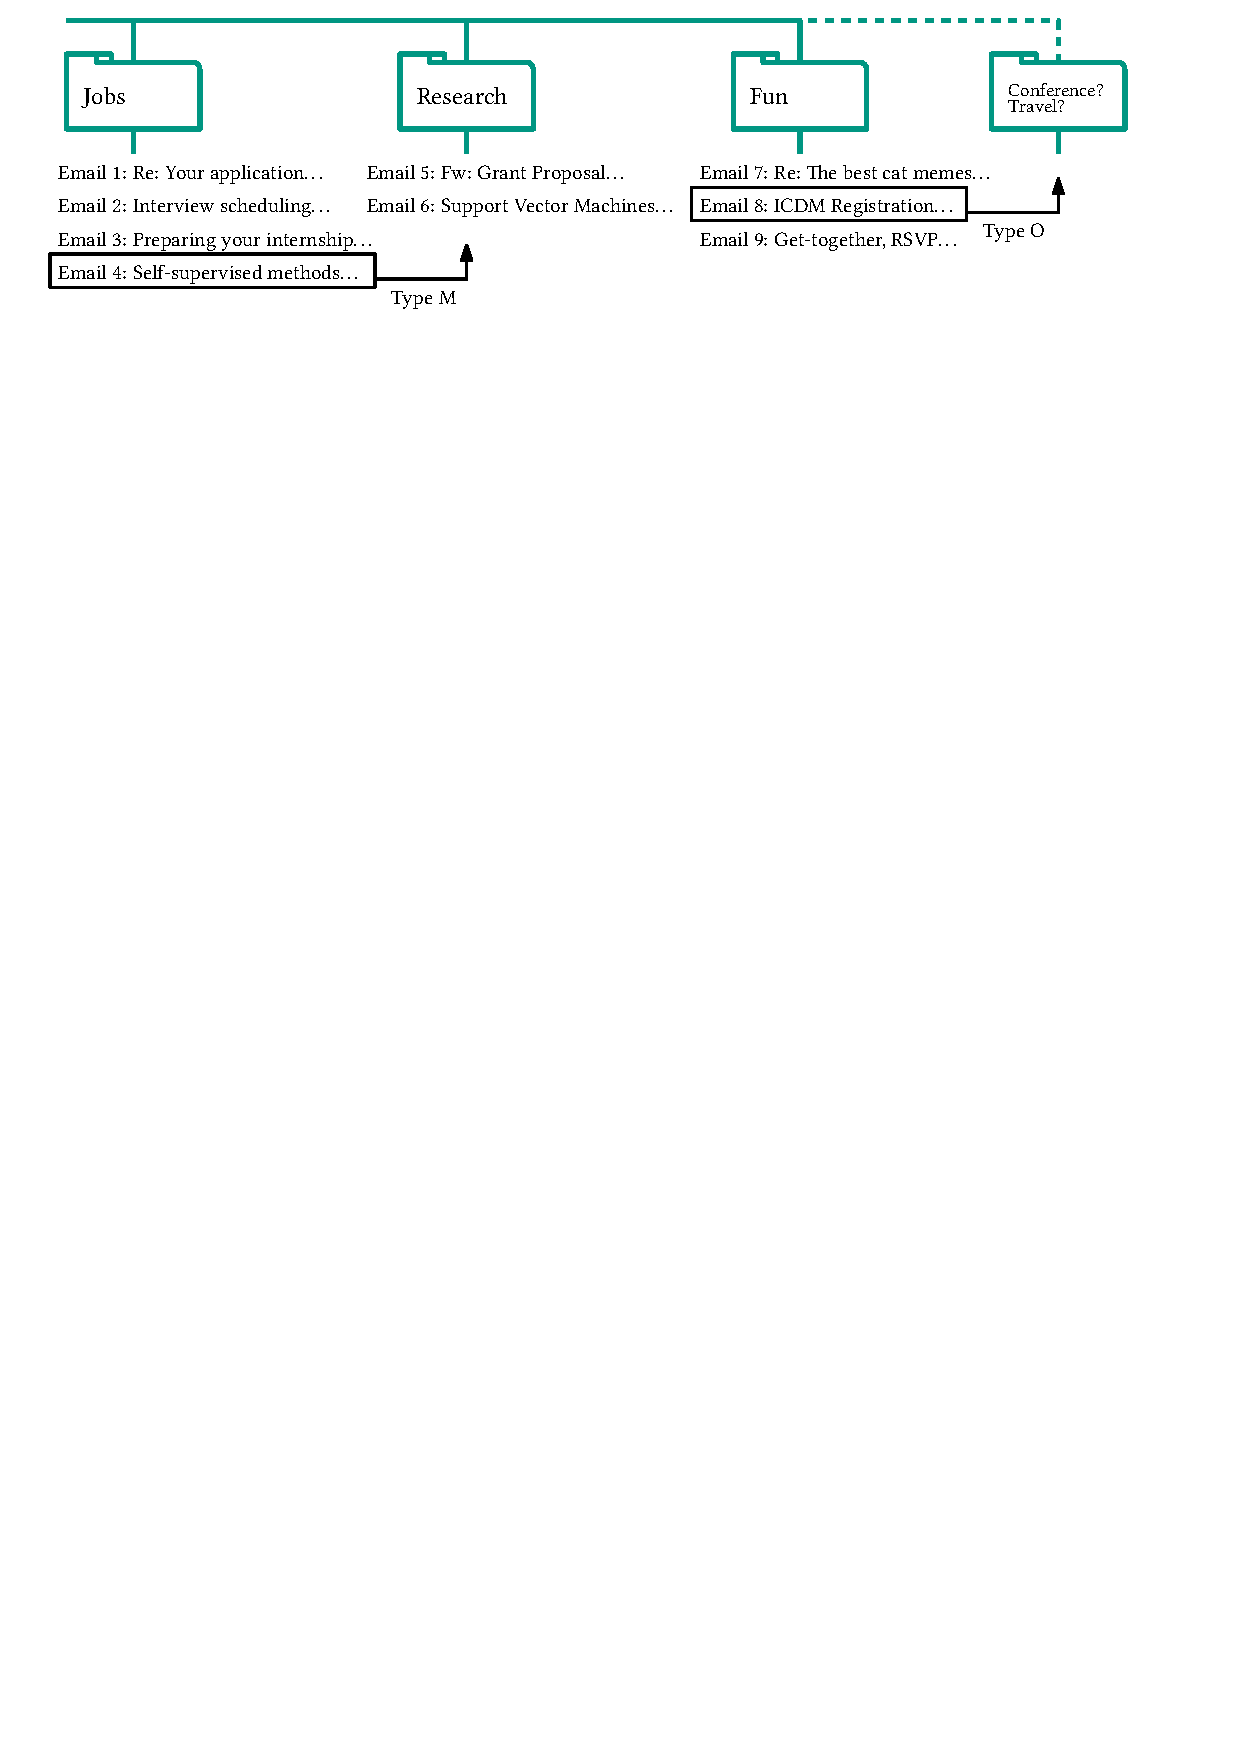
\includegraphics[width=\linewidth]{part1-figures/illustrative_example_2-compressed.pdf}
	\caption{Email Archiving: An Illustrative Example.}
	\label{fig:illustrative_example}
\end{figure}

Detecting documents classified erroneously is difficult \cite{DBLP:journals/tnn/FrenayV14, DBLP:series/isrl/2015-72}. This is because folder structures typically are domain-specific and are user-defined taxonomies. At the same time, documents can be misplaced in numerous, unforeseeable ways, which may or may not be folder-specific. 
So seeing this problem as a supervised one -- where a ground truth is available -- would be inadequate. Next, orthogonally to this `semantic' level, two types of errors/outliers can occur: \textbf{(O) Out-of-distribution}: A document does not belong to any existing folder --- the user should create a new class. % for Email 8.)
\textbf{(M) Misclassification}: A document belongs to another folder in the directory --- the user misclassified it.

We illustrate this in Figure~\ref{fig:illustrative_example}, with (fictitious) emails ordered into folders by a user: Email 4 is a Type~M outlier, as it belongs to the folder `Research'. Email 8 in turn is a Type~O outlier, because it does not fit into any existing folder --- we should create a new one. 
Intuitively, a document is a Type~O outlier when it does not appear to be similar to documents of any single class. 
In contrast, a document is a Type~M outlier when it appears to be most similar to documents from another class. 

In this work, we focus on mining text outliers in document directories. %Doing so improves existing text archives and supports the annotators. 
It is difficult  because documents are outlying w.r.t.\ their semantics, which is not easy to capture (even for humans). 
An additional issue, which makes this contribution unique, is that both outlier types must be detected jointly. 
Namely, the existence of one type harms the detection of the other one. 
The noise introduced by Type~M outliers hinders the detection of Type~O outliers. Conversely, Type~O outliers may be detected as Type~M by mistake, leading to a poor treatment of such outliers.
Existing methods only deal with one of these outlier types, cf.\ Section~\ref{relatedwork:MiningTextOutliers}. Interestingly, we show that the joint detection of both outlier types leads to better performance for each type than approaches only dealing with one of them. 
%This is suboptimal, as we will show.% in our study. 

To solve this problem, we propose a new approach to detect text outliers, which we name \gls{kj-NN}\footnote{See also \url{https://youtu.be/6dl3ZBxB3f0} for a 18-minute talk about our contribution.}. Our approach leverages similarities of documents and phrases, based on state-of-the-art embedding methods \cite{meng2019spherical}, to detect both Type~O/M outliers. By extracting semantically relevant labels and the documents similar to each outlier, it also supports interpretability. Our approach is efficient and robust to large proportions of erroneous labels thanks to a `self-supervision' mechanism, which estimates the relevance of the original labels. 
%Our idea is to weigh each decision by the relevance of neighbouring documents. A document is said to be relevant w.r.t.\ a given class when its semantics, characterised by its closest phrases in the embedding space, is representative of its class. 
Our experiments show that our approach improves the current state of the art by a large margin while delivering interpretable results. In the next section, we introduce our notation. 

\subsubsection{Notation}

Let $\gls{Doc} = \{\gls{d}_1, \gls{d}_2, \dots, \gls{d}_{|\gls{Doc}|}\}$ and $\gls{Phr} = \{\gls{p}_1, \gls{p}_2, \dots, \gls{p}_{|\gls{Phr}|}\}$ 
be a set of documents and phrases. We define $\gls{O} = \gls{Doc} \cup \gls{Phr}$ as the set of all text objects. 

A common practice in the community is to project each text object in an $n$-dimensional embedding space as a preprocessing step. In this paper, we use a recent technique \cite{meng2019spherical} capable of projecting both words and documents into the same embedding space, i.e., each object $\gls{o}$ has an embedding vector representation $\gls{V}: \gls{O} \mapsto \mathbb{R}^n$ with $n$ dimensions, with typically $n \geq 100$. The vectors are all normalised, thus $\| \gls{V}(\gls{o}) \| = 1,~\forall \gls{o} \in \gls{O}$.

We quantify the similarity between a pair of phrases, documents or phrases/documents with a function $\gls{Sim}: \gls{O}^2 \mapsto [0,1]$ where $1$ is the highest possible similarity (identity) and $0$ is the lowest one. In our setting, $\gls{Sim}$ is the normalised cosine similarity: 

\begin{equation}
\label{eq:cosinesimilarity}
\gls{Sim}(\gls{V}(\gls{o}_i), \gls{V}(\gls{o}_j)) = \frac{\gls{V}(\gls{o}_i) \cdot  \gls{V}(\gls{o}_j) + 1}{2} \quad \forall (\gls{o}_i, \gls{o}_j) \in \gls{O}^2
\end{equation}

For simplicity, we equivalently refer to the vectorial representation of each object, i.e., $\gls{o} \equiv \gls{V}(\gls{o})$, in what follows. We also assume that there exists an initial classification of documents into a set of classes $\gls{C} = \{\gls{c}_1, \dots, \gls{c}_{|\gls{C}|}\}$, expressed as a function $\mathit{\gls{y}}: \gls{Doc} \mapsto \gls{C}$. 

Our self-supervision mechanism relies on estimating the \textit{representativeness} of each phrase $\gls{p} \in \gls{Phr}$ w.r.t.\ each class $\gls{c} \in\gls{C}$. We denote it as a function $\mathit{\gls{r}}: \gls{Phr} \times \gls{C} \mapsto \mathbb{R}^+$. 

In Chapter \ref{chapter:textoutlier}, we extensively describe our approach and experiments. Note that for this study, we restricted our experiments to static text repositories. Nonetheless, our other contributions facilitate the extension of our approach to streams of text, e.g., news or twitter feeds. In that respect, one may see Chapter \ref{chapter:textoutlier} as preliminary work. Applying our methods for Knowledge Discovery in streams of text is future work (cf. Chapter \ref{chapter:futurework}). 


\chapter{Related Work}
\glsresetall
\label{chapter:relatedwork}

This chapter reviews the related work for each of our contributions.

\section{Estimating Dependency}

Estimating the dependency, or `correlation', between two or more variables, is a fundamental topic in data analysis and has motivated research for more than a century. Many bivariate measures exist, e.g., \cite{10.2307/1412159, 10.2307/1412159, 10.2307/2332226, Reshef1518}. Some of them also target at quantifying the association between two vectors which are possibly multivariate \cite{DBLP:conf/nips/GrettonFTSSS07, 10.2307/27801540, DBLP:conf/nips/Lopez-PazHS13, DBLP:conf/icml/BelghaziBROBHC18}. 
However, they can only quantify the dependency between two entities -- not between several ones (\hyperlink{R1}{\textbf{R1}}). %Note: this is known as canonical dependency estimation approaches 
They also may have other drawbacks. 
The Pearson correlation coefficient, for instance, is parametric  (\hyperlink{R4}{\textbf{R4}}), targets at linear dependencies (\hyperlink{R2}{\textbf{R2}}) and is only applicable to numerical data (\hyperlink{C5}{\textbf{C5}}).

There are attempts to extend bivariate dependency measures to the multivariate case. For example, there exists an extension of Spearman's $\rho$ to multidimensional data (\gls{MS}), but it is limited to monotonous relationships (\hyperlink{R2}{\textbf{R2}}). 
Several authors also propose multivariate extensions of \gls{MI} \cite{DBLP:journals/jcns/TimmeAFB14}. For example, \gls{II} \cite{DBLP:journals/tit/McGill54} quantifies the `synergy' or `redundancy' in a set of variables. Similarly, \gls{TC} \cite{DBLP:journals/ibmrd/Watanabe60} quantifies the total amount of information. 
However, information-theoretic measures are difficult to estimate, as they require knowledge about the underlying probability distributions. Density estimation methods, either based on kernels, histograms or local densities, 
all require setting unintuitive  parameters (\hyperlink{R3}{\textbf{R3}}) and may be computationally expensive (\hyperlink{C1}{\textbf{C1}}). Next, with many attributes, density estimation becomes meaningless due to the \textit{curse of dimensionality} \cite{bellman1957}. 
Information-theoretic measures also are difficult to interpret (\hyperlink{R5}{\textbf{R5}}), since they usually correspond to a number of bits or nats, which is theoretically unbounded. 

More recently, \gls{CMI},  \gls{MAC}, \gls{UDS},
\gls{UMC} and \gls{IID} were proposed as multivariate dependency measures. They are remotely related to concepts from information theory, as they rely on the so-called \gls{CE}. 
However, these measures are computationally expensive (\hyperlink{C1}{\textbf{C1}}) and unintuitive %to use
(\hyperlink{R3}{\textbf{R3}}). 
They also are difficult to interpret, because their theoretical maximum and minimum vary with the number of attributes (\hyperlink{R5}{\textbf{R5}}). 

Another approach, \gls{HiCS}, is somewhat similar to ours, \gls{MCDE}.
It uses \textit{subspace slicing} as a heuristic to quantify the potential of subspaces to contain outliers. Yet \gls{HiCS} only addresses static numerical data, and its suitability as a dependency estimator is not known. 

Also, most dependency estimators are designed to deal with numerical data only, and one assumes that all relevant observations are available during estimation. In the real world, however, data often consists of an open-ended, ever-evolving stream of measurements or indicators of various types, e.g., numerical, ordinal, or categorical observations.

The current state of the art to handle heterogeneity (\hyperlink{C5}{\textbf{C5}}) is to rely on discretisation, using methods such as the one proposed by \cite{DBLP:conf/ijcai/FayyadI93}. %,  as a pre-processing step. 
Then one can compute an information-theoretic measure, as in \cite{DBLP:conf/ssdbm/NguyenMAB14}. However, any discretisation essentially results in an information loss and may not work as dimensionality increases. %, because of data sparsity.

A recent line of work focuses on estimating \gls{MI} on numerical data streams. \gls{MISE} is a data summarisation technique to estimate \gls{MI} over arbitrary time windows. 
\cite{DBLP:conf/edbt/VollmerRB18} provide dynamic data structures to maintain \gls{MI} over a sliding window. % and provide lower bounds for the quality of estimates. 
\cite{DBLP:conf/edbt/VollmerB19} extend this method to propose an anytime estimator for \gls{MI}, with confidence bounds. 
However, the resulting estimates inherit the qualities and caveats from \gls{MI}. 

\section{Monitoring}

We refer to `monitoring' as the continuous surveillance of statistics in a multidimensional, potentially high-dimensional data stream. The existing approaches for monitoring statistics in streams fall into two classes: incremental and approximation schemes. 

\textbf{Incremental Schemes:} One can monitor statistics on  streams incrementally via a forgetting mechanism, to discard past observations. 
The approaches are usually based on a sliding window \cite{DBLP:conf/sdm/BifetG07, DBLP:conf/edbt/VollmerRB18} or a decaying factor \cite{koychev2000gradual, DBLP:journals/ida/Klinkenberg04, DBLP:conf/ssdbm/SchubertG18}. 
However, not every statistic can be computed incrementally, and the schemes only handle the computation of a single statistic, not of multiple ones. 

\textbf{Approximation Schemes:} Another line of research is approximating the statistics via sampling strategies \cite{DBLP:conf/soda/BabcockDM02, DBLP:conf/sac/BoidolH17, DBLP:conf/ssdbm/ArzamasovBR19} or data transformations, such as Fourier \cite{DBLP:conf/vldb/ZhuS02, DBLP:conf/iisa/SeliniotakiTCT14} or wavelet \cite{DBLP:journals/vldb/ChakrabartiGRS01, DBLP:conf/kdd/GuhaH05} transform. Other approaches explicitly target at high dependency \cite{DBLP:journals/ngc/KarguptaPKS06, DBLP:conf/kdd/ZhouX08}. However, most methods work only for specific statistics, e.g.,  Pearson's correlation, which limits their applicability to linear dependencies.  

Work on change detection also is related, as detecting whenever a change occurs in the stream helps with monitoring. \cite{DBLP:conf/sdm/NguyenV16a}, \cite{DBLP:conf/kdd/ReisFMB16} or \cite{DBLP:journals/tkde/BlancoCRBDM15} all aim to detect sudden changes. However, these approaches do not apply to stream data or require labels, which make them unsuitable for the high-dimensional streaming setting in general and further applications, e.g., predictive maintenance. % In Section \ref{bandits}, we give more details about how we intend to approach this problem. 

Our approach, \gls{S-MAB}, does not fall into these categories, since we target at monitoring virtually any statistics; the estimates are exact, but our algorithm decides when to update them. To do that, we show that our method can also leverage change detectors, such as \gls{ADWIN}. Thus, our contribution is orthogonal to the existing work. For a broader overview of stream monitoring methods, see \cite{DBLP:books/daglib/0030859}.

Since our approach bases on bandit theory, the existing bandit models also are related. Work on bandits traces back to \cite{Thompson1933}, with the design of clinical trials. %In 1953, behavioural psychologists \cite{Bush1953} coined the term \textit{bandit} in analogy to the well-known slot machines. 
The theoretical guarantees of bandits remained unknown until recently \cite{DBLP:journals/eccc/ECCC-TR00-068,DBLP:journals/ml/AuerCF02,Garivier2008, DBLP:conf/alt/KaufmannKM12}. Our work builds on several facets of bandits, which have been studied separately, such as anytime bandits \cite{DBLP:conf/soda/Kleinberg06, DBLP:conf/icml/DegenneP16}%slivkins2008adapting,garivier2018kl
, \gls{MP-MAB} \cite{1104491,DBLP:conf/alt/UchiyaNK10, DBLP:conf/icml/KomiyamaHN15} %agrawal1990multi 
and bandits in non-static environments \cite{DBLP:journals/siamcomp/AuerCFS02, DBLP:conf/colt/SlivkinsU08, DBLP:conf/alt/GarivierM11}. %However, to the best our knowledge, we are the first to consider all of these "complications" together. 

One can see the \gls{S-MAB} as an extension of the \gls{MP-MAB}, with the novelty that the player must control the number of plays over time. 
In particular, we build on the work from \cite{DBLP:conf/icml/KomiyamaHN15}.
It shows that \gls{MP-TS} has optimal regret while being efficient. We compare our results with other multiple-play models, such as variants of the celebrated \gls{UCB} and the \gls{Exp3}, namely \gls{CUCB}, \gls{MP-KL-UCB} and \gls{Exp3.M}. 

Our problem is different from the profitable bandits \cite{DBLP:conf/acml/AchabCG18} since they aim at maximising a static notion of profit -- as opposed to efficiency -- which boils down to finding the individual arms for which the rewards exceed the costs in expectation. 
Moreover, our problem is more challenging than the \gls{MP-MAB} and its extension called \gls{CMAB} in that we are interested in a set of arms where the model parameters $\mu_i$ satisfy an efficiency constraint (see Eq. \eqref{eq1}), and the algorithm needs to estimate them.

\glsunset{MAB}
The \gls{S-MAB} also is related to the budgeted \gls{MAB} model \cite{DBLP:conf/aaai/LongCCRJ10, DBLP:conf/ijcai/XiaQMYL16}%xia2015thompson
, because it aims at maximising a notion of efficiency, i.e., the ratio of the reward to the cost of playing arms.
In our case, the total number of plays -- the `budget' -- is not an external constraint. Instead, the \gls{S-MAB} decides how many arms to play based on its observations of the environment. %We also make the assumption that each arm is associated to the same cost. 

%Our approach also is related to \textit{combinatorial bandit} \cite{cesa2012combinatorial, chen2013combinatorial} and \textit{thresholding bandits} (link to clarify). % also restless bandits (Improving Online Marketing Experiments with Drifting Multi-armed Bandits)
%EF: Since our approach is "two-step", I find it a bit similar to Adapt-Eve too (which does not have any theoretical analysis, even if very good in practice)
%EF: The approach also shares similarities with Viappiani, Paolo. "Thompson sampling for bayesian bandits with resets." International Conference on Algorithmic DecisionTheory. (at difference of scaling and being multiple play, using ADWIN and not a particle filter)
% Also the multiple-play aspects is close to the "Non-Stochastic Bandit Slate Problems" (kale). 
%See also "A Change-Detection based Framework for Non-stationary Multi-Armed Bandit Problem") (UCB + Change point detection)
% Also,  SAO: Stochastic and Adversarial Optimal (Combines UCB1 and Exp3)
% "Surveillance in an Abruptly Changing World via Multiarmed Bandits" is somewhat related to the scaling bandit

% "On Upper-Confidence Bound Policies for Switching Bandit Problems" (Garivier11) is an archetypal example that considered abrupt changes, while "Slivkins, A., Upfal, E.: Adapting to a changing environment: the brownian restless bandits" considers distribution  of rewards that changes continuously
% According to "Hartland, C., Gelly, S., Baskiotis, N., Teytaud, O., Sebag, M.: Multi-armed bandit, dynamic environments and meta-bandits (2006)" standard soft-max and UCB policies are not appropriate for abruptly changing environments
% Some work on correlation monitoring: 
% COREQ: https://hpi.de/mueller/coreq.html
% FMC: "Minefleet: The vehicle data stream mining system for ubiquitous environments"
% Statstream: "Statstream: Statistical monitoring of thousands of data streams in real time"
% PeakSim: "Stream correlation monitoring for uncertainty-aware data processing systems"

Bandits have readily been applied to many real-world applications, such as packet routing \cite{DBLP:conf/stoc/AwerbuchK04}, online advertising \cite{DBLP:conf/nips/ChakrabartiKRU08}, recommendation systems \cite{DBLP:conf/www/LiCLS10}, robotic planning \cite{DBLP:conf/cdc/SrivastavaRL14} and resource allocation \cite{DBLP:journals/pvldb/LiZLWZ18}. 
Nonetheless, the application of bandits to monitoring (see Example \ref{bandit:runningexample}) has received much less attention.
For an overview of bandit algorithms, we refer the reader to recent surveys \cite{DBLP:journals/ftml/BubeckC12, DBLP:journals/corr/BurtiniLL15, lattimore18}.   

%\begin{itemize}
%	\item Useful fundamentals and formalisms: \cite{Bubeck2012}
%	\item Useful survey: \cite{burtini2015survey}
%	\item Non-static: Discounted UCB / Sliding Window UCB \cite{Garivier2008}, surveillance (switching window) \cite{srivastava2014surveillance}
%	\item Contextual Bandits: survey \cite{zhou2015survey}, efficient optimal learning \cite{dudik2011efficient}, mobile health \cite{tewari2017ads}
%	\item Adversarial and multiple play: \cite{uchiya2010algorithms}
%	\item Multiple play: ad placement \cite{louedec2015multiple}, thompson sampling \cite{komiyama2015optimal}, budgeted \cite{xia2016budgeted}
%	\item Budgeted: budget-limited (Ph.D. thesis) \cite{tran2012budget}, finite budget analysis \cite{xia2017finite}, many-arm \cite{li2017infinitely}, thompson sampling \cite{xia2015thompson}
%	\item Adversarial: adaptive algorithms \cite{wei2018more}, Exp3++ \cite{seldin2017improved}, Boltzmann exploration \cite{cesa2017boltzmann}
%	\item Anytime: \cite{besson2018doubling}, online portfolio choice \cite{shen2015portfolio}
%	\item Non-static: \cite{allesiardo2017non}, restless (website optimization) \cite{burtini2015improving}, restless (seminal paper) \cite{whittle1988restless} 
%	\item Following-the-perturbed-leader: \cite{hutter2005adaptive}
%\end{itemize}

\section{Knowledge Discovery}

% Maybe relevant: Sliding window-based fault detection from high-dimensional data streams L Zhang, J Lin, R Karim
% Maybe relevant: An angle-based subspace anomaly detection approach to high-dimensional data: With an application to industrial fault detection L Zhang, J Lin, R Karim
% Maybe relevant: An adaptive algorithm for anomaly and novelty detection in evolving data streams Mohamed-Rafik Bouguelia, Slawomir Nowaczyk & Amir H. Payberah 
% Maybe also: Deep Incremental Learning for Big Data Stream Analytics SA Alex, JJV Nayahi 
% Maybe also: An improvement growing neural gas method for online anomaly detection of aerospace payloads L Song, T Zheng, J Wang, L Guo

Because of the unsupervised nature of tasks in high-dimensional streams, knowledge discovery mainly is limited to two classes of applications: outlier/anomaly detection and clustering. As mentioned in recent studies \cite{DBLP:conf/ssdbm/KriegelKNZ11,DBLP:conf/sdm/NtoutsiZPKK12}, little effort was devoted so far to the discovery of patterns in high-dimensional data streams. Most contributions focus instead on only one of the two aspects: high-dimensionality or data streams. 

While recent studies, such as \cite{DBLP:conf/vldb/AggarwalHWY04, DBLP:conf/icde/ZhangGW08, DBLP:conf/ssdbm/KriegelKNZ11, DBLP:conf/sdm/NtoutsiZPKK12}, attempt to address high-dimensional data streams, the dimensionality in benchmarks is limited -- usually, to less than $50$ dimensions. Thus, whether those approaches can scale is not known. Recent surveys \cite{DBLP:journals/tkde/GuptaGAH14, DBLP:journals/jcst/AminiTS14} provide a good overview of the state-of-the-art methods for Knowledge Discovery in data streams w.r.t. the task of outlier detection and clustering.

While addressing every Knowledge Discovery problem is out of the scope of this dissertation, the fundamental nature of our contributions helps towards this goal. We focus in particular on two Knowledge Discovery tasks: `Subspace Search in Data Streams' and `Mining Text Outliers', for which we detail the related work hereafter. 

\subsection{Subspace Search in Data Streams}

Many methods for subspace search exist, but almost all of them are either coupled to a specific Data Mining algorithm or are limited to the static setting. 
For example, various approaches for streams \cite{DBLP:conf/ideas/KontakiPM06, DBLP:conf/icdm/ZhangLW07, DBLP:conf/icde/ZhangGW08, DBLP:conf/icde/Aggarwal09a} % vanea2012instant
only tend to work with a given static algorithm. Other methods in turn \cite{DBLP:conf/icde/KellerMB12, DBLP:conf/sdm/BohmKMNV13, DBLP:conf/bigdataconf/NguyenMB13, DBLP:conf/sdm/NguyenMV16, DBLP:conf/aaai/WangRNBMX17, DBLP:journals/ijdsa/TrittenbachB19} decouple the search from the actual task, but none of them can handle streams. The existing work on subspace search mostly focuses on individual applications \cite{DBLP:journals/sigkdd/ParsonsHL04, DBLP:journals/tkdd/KriegelKZ09, DBLP:journals/sadm/ZimekSK12}, e.g., clustering or outlier detection, while `general-purpose' subspace search has received less attention. 

To our knowledge, there exist two proposals to extend subspace search to streams in a general way: HCP-StreamMiner \cite{vanea2012instant} and Stream\gls{HiCS} \cite{becker2016concept}. 
But these approaches boil down to a periodic repetition of the procedure in \cite{DBLP:conf/icde/KellerMB12} on synopses of the stream. 
We will see that our method outperforms these approaches. %, while requiring much less computation. 
\gls{GMD} is the approach most similar to ours. 
It uses a so-called contrast measure \cite{DBLP:conf/icde/KellerMB12} to quantify the interestingness of a given subspace and builds a set of subspaces via a greedy heuristic. 
However, \gls{GMD} assumes static data.

Subspace search has been used in the past to improve the results of Data Mining tasks such as outlier detection \cite{DBLP:conf/icde/ZhangGW08, DBLP:conf/icde/KellerMB12,  DBLP:journals/ijdsa/TrittenbachB19}. The authors compare their results with full-space static outlier detectors. %There exists a plethora of methods for outlier detection, both in the static and streaming setting. 
We perform an analogous evaluation in the streaming setting and compare our results against several baselines and state-of-the-art stream outlier detectors, such as xStream \cite{10.1145/3219819.3220107} and \gls{RS-Stream}. See \cite{DBLP:journals/tkde/GuptaGAH14} for a survey of outlier detection in streams.

\subsection{Mining Text Outliers}
\label{relatedwork:MiningTextOutliers}
%In this section, we review existing studies for document-level outlier detection. 
\glsunset{kj-NN}

To our knowledge, none of the existing methods handles both outlier types. 
So we categorise related work into two classes: (1) Type~O and (2) Type~M outlier detectors. 

\textbf{Type~O outlier detectors.} Type~O is the standard definition of outliers, and detecting such outliers has been studied for decades. 
Conventional outlier detection approaches typically fall into the following classes: distance-based \cite{knox1998algorithms,ramaswamy2000efficient}, neighbour-based \cite{DBLP:conf/sigmod/BreunigKNS00,kriegel2008angle}, probabilistic-based \cite{kim2012RKDE,tipping1999PPCA} and subspace-based methods \cite{DBLP:journals/kais/SatheA18,lazarevic2005feature,muller2012outlier,DBLP:conf/icde/KellerMB12,kriegel2012outlier}. Examples of conventional methods are the well-known \gls{LOF} or, more recently, \gls{RS-Hash}. However, textual data is typically extremely sparse, and thus few of the above proposals can detect outlier documents, as they do not model semantics.

There exist a few methods addressing text outliers: \cite{DBLP:conf/emnlp/ZhuangWTKH17} proposes a generative approach, which models the embedding space as a mixture of von \gls{vMF} distributions. They identify `outlier regions' that deviate from the majority of the embedded data. \acrshort{TONMF} \cite{DBLP:conf/sdm/KannanWAP17}, a Non-negative Matrix Factorisation (NMF) approach, bases on block coordinate descent optimisation. 
Recently, Ruff et al.\ proposed \gls{CVDD}, a one-class classification model leveraging pre-trained language models and a multi-head attention mechanism. However, all of these methods treat outlier detection as a one-class classification problem, i.e., they try to describe an `abnormal' class and a `normal' class; none of them addresses Type~M outliers. 

\textbf{Type~M outlier detectors.} Type~M outliers represent misclassified text. While this type of outlier is ubiquitous, it has received little attention so far. 
Few publications try to address the problem directly. 
Traditional supervised text classification methods, assuming the ground truth to be error-free, have no choice but to tolerate Type~M outliers during training. 
While one can extend the existing supervised document classification models (e.g., \cite{DBLP:conf/emnlp/Kim14, DBLP:conf/eacl/SchwenkBCL17, DBLP:conf/acl/ZhouSTQLHX16, DBLP:conf/aaai/LaiXLZ15}) to mitigate the effect of Type~M outliers, they are in turn not helpful to detect Type~O outliers. 

As we explained earlier, the existence of both outlier types calls for methods that can detect them simultaneously. In that respect, our method, \gls{kj-NN}, is the first of its kind. In our experiments, we compare our approach against the methods above and show that we outperform all of them. We refer the reader to \cite{DBLP:books/sp/Aggarwal2013} for an extensive overview of existing outlier detection methods. 

%Some further elements: 
%Novelty detection \cite{zhang2005probabilistic, zhang2002novelty, kasiviswanathan2012online, kasiviswanathan2013novel} [Handling type A only]. 
%\cite{DBLP:journals/sigkdd/SunH12} identifies our focus as an important challenge. 
%Document clustering, classification [...]. Clustering is often useful for Type A outliers, while classification for Type B. 
%WeSTClass \cite{DBLP:conf/cikm/MengSZ018}, WeSHClass \cite{DBLP:conf/aaai/MengSZH19} targets at text classification with weak supervision [No outlier detection, i.e., no Type A, different setup]. 
%Zero-shot classification \cite{DBLP:conf/naacl/ZhangLG19} [?]. 
%\cite{barigou2016improving} is related work, it uses k-NN for text classification (TODO: clarify the relationship). 
%Maybe rule out the effort made in the crowdsourcing community as we may not use any kind of majority voting (no consensus possible). 
%Maybe discuss that kNN can be used as an outlier detection method, but quite in a different way (usually extensions like LOF \cite{DBLP:journals/datamine/CamposZSCMSAH16}). 
%Topic modelling [?]. 
%Graph outlier ranking method \texttt{GOutRank} \cite{DBLP:conf/icde/MullerSMB13}. 
%Community distribution outlier detection CDODA \cite{DBLP:conf/pkdd/GuptaGH13}. 
%Embedding methods: JoSE \cite{meng2019spherical} on which we are building, probably need to consider Doc2Vec \cite{DBLP:conf/icml/LeM14} also. 
%\item \texttt{RankClus} \cite{DBLP:conf/edbt/SunHZYCW09}, historical word on heteregeneous information networks (bi-typed), as well as its follow-up \texttt{NetClus} \cite{DBLP:conf/kdd/SunYH09} (star-schema)
%\item \texttt{KnowSim} \cite{DBLP:conf/icdm/WangSLZH15} similarity measure on HIN
% See \url{https://github.com/brightmart/text_classification} for some type B baselines.